\documentclass[aspectratio=169]{beamer}
\geometry{paperwidth=320mm,paperheight=180mm}
\usepackage{fontspec}
\setmainfont[Path=fonts/,FontIndex=7,BoldFont=AvenirNext.ttc,BoldFeatures={FontIndex=2},ItalicFont=AvenirNext.ttc,ItalicFeatures={FontIndex=4},BoldItalicFont=AvenirNext.ttc,BoldItalicFeatures={FontIndex=3}]{AvenirNext.ttc}
\setsansfont[Path=fonts/,FontIndex=7,BoldFont=AvenirNext.ttc,BoldFeatures={FontIndex=2},ItalicFont=AvenirNext.ttc,ItalicFeatures={FontIndex=4},BoldItalicFont=AvenirNext.ttc,BoldItalicFeatures={FontIndex=3}]{AvenirNext.ttc}
\newfontfamily\heavy[Path=fonts/,FontIndex=2]{AvenirNext.ttc}
\setmonofont[Path=fonts/,BoldFont=JetBrainsMono-Bold.ttf,ItalicFont=JetBrainsMono-Italic.ttf,Contextuals=NoAlternate,Ligatures=NoCommon]{JetBrainsMono-Regular.ttf}
\usepackage{xcolor,graphicx,tikz,booktabs,tabularx,listings,amsmath}
\usetikzlibrary{arrows.meta,positioning}
\definecolor{paper}{HTML}{FFFFFF}
\definecolor{ink}{HTML}{252525}
\definecolor{teal}{HTML}{252525}
\definecolor{orange}{HTML}{777777}
\definecolor{wash}{HTML}{EAEAEA}
\definecolor{quiet}{HTML}{666666}
\definecolor{lightink}{HTML}{D0D0D0}
\definecolor{codepaper}{HTML}{F6F6F4}
\lstset{language=Python,basicstyle=\ttfamily\fontsize{9.5}{13}\selectfont\color{ink},keywordstyle=\bfseries\color{ink},commentstyle=\itshape\color{quiet},stringstyle=\color{ink},showstringspaces=false,columns=fullflexible,keepspaces=true,breaklines=true,breakatwhitespace=true,numbers=none,upquote=true,aboveskip=8pt,belowskip=6pt}
\hyphenpenalty=4000
\emergencystretch=3em
% The same two-line navigation and fine rule as the reference, without a candy motif.
\newcommand{\guideheader}[2]{\begin{tikzpicture}[remember picture,overlay]
\node[anchor=north west,inner sep=0,text width=176mm] at ([xshift=16mm,yshift=-7mm]current page.north west) {\fontsize{8.5}{10}\selectfont\color{quiet}#1};
\node[anchor=north west,inner sep=0,text width=176mm] at ([xshift=16mm,yshift=-11.5mm]current page.north west) {\heavy\fontsize{10}{12}\selectfont\color{ink}#2};
\draw[lightink,line width=.4pt] ([xshift=16mm,yshift=-17mm]current page.north west)--([xshift=192mm,yshift=-17mm]current page.north west);
\end{tikzpicture}}

\usepackage{colortbl}
\usetikzlibrary{fit}
\newsavebox{\codebox}
\setbeamercolor{normal text}{fg=ink,bg=paper}
\setbeamertemplate{navigation symbols}{}\setbeamertemplate{footline}{}\setbeamertemplate{headline}{}
\begin{document}
\begin{frame}[plain,fragile]\begin{tikzpicture}[remember picture,overlay,x=1cm,y=1cm]\begin{scope}[shift={(current page.south west)}]
\node[anchor=north west,inner sep=0pt,text width=29cm,align=left,text=teal,font=\fontsize{16}{\dimexpr16pt*6/5\relax}\selectfont] at (1.5,16.5) {\heavy LESSON 2};
\node[anchor=north west,inner sep=0pt,text width=29cm,align=left,text=ink,font=\fontsize{46}{\dimexpr46pt*6/5\relax}\selectfont] at (1.5,14.4) {\heavy Dice and\\Grid Paths};
\node[anchor=north west,inner sep=0pt,text width=29cm,align=left,text=quiet,font=\fontsize{22}{\dimexpr22pt*6/5\relax}\selectfont] at (1.5,9.3) {Count the ways to arrive};
\node[anchor=south,inner sep=0] at (16,2.3) {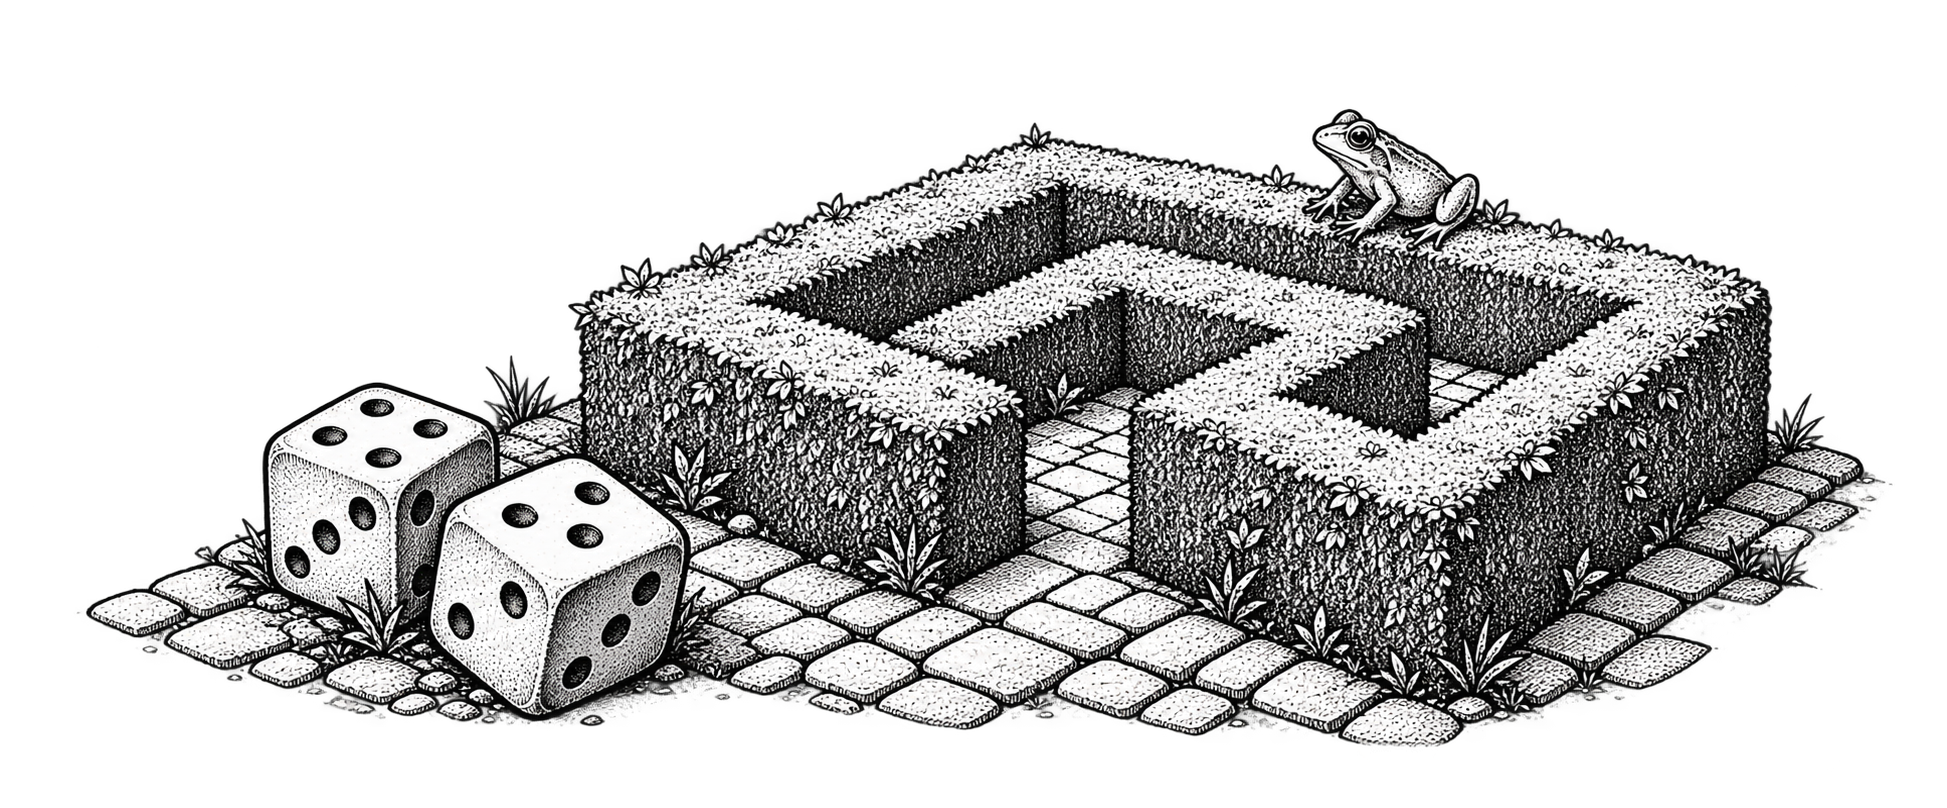
\includegraphics[width=27cm,height=6cm,keepaspectratio]{assets/cover.png}};\node[anchor=west,inner sep=0] at (1.5,1) {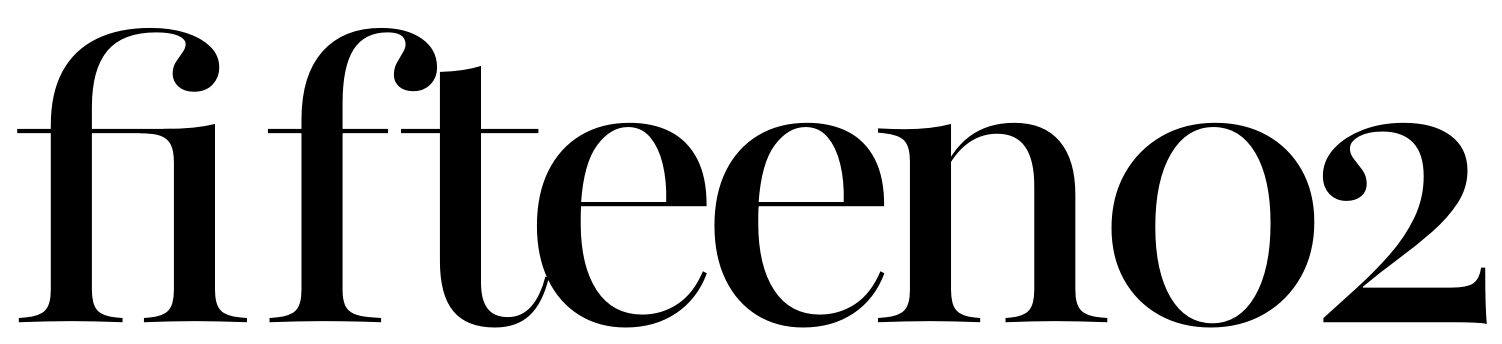
\includegraphics[width=3.8cm]{assets/logo.png}};\node[anchor=east,inner sep=0] at (30.5,1) {
\includegraphics[width=5.5cm]{assets/julians-pathfinder-monochrome.pdf}};
\node[anchor=north west,inner sep=0pt,text width=1cm,align=left,text=quiet,font=\fontsize{11}{\dimexpr11pt*6/5\relax}\selectfont] at (15.8,0.8) {\insertframenumber};
\node[anchor=north west,inner sep=0pt,text width=12cm,align=left,text=ink,font=\fontsize{14}{\dimexpr14pt*6/5\relax}\selectfont] at (18,16.5) {\href{https://colab.research.google.com/github/fifteen02/julians-pathfinder/blob/main/Lesson\%202/lesson.ipynb}{\underline{Open this lesson in Google Colab}}};
\end{scope}\end{tikzpicture}
\end{frame}

\begin{frame}[plain,fragile]\begin{tikzpicture}[remember picture,overlay,x=1cm,y=1cm]\begin{scope}[shift={(current page.south west)}]
\node[anchor=north west,inner sep=0pt,text width=29cm,align=left,text=quiet,font=\fontsize{13}{\dimexpr13pt*6/5\relax}\selectfont] at (1.5,16.9) {\heavy LESSON 2 / TODAY};
\node[anchor=north west,inner sep=0pt,text width=1cm,align=left,text=quiet,font=\fontsize{11}{\dimexpr11pt*6/5\relax}\selectfont] at (30,0.8) {\insertframenumber};
\node[anchor=north west,inner sep=0pt,text width=29cm,align=left,text=quiet,font=\fontsize{18}{\dimexpr18pt*6/5\relax}\selectfont] at (1.5,15.4) {\heavy MAIN IDEA};
\node[anchor=north west,inner sep=0pt,text width=29cm,align=left,text=ink,font=\fontsize{40}{\dimexpr40pt*6/5\relax}\selectfont] at (1.5,14.3) {\heavy Count the ways to arrive.};
\node(idea)[anchor=north west,inner sep=0pt,text width=28cm,align=left,text=ink,font=\fontsize{24}{\dimexpr24pt*6/5\relax}\selectfont] at (1.5,11.9) {To count the ways to reach a target, split them by their last move and add the counts for where that move started.};
\node[anchor=north west,inner sep=0pt,text width=28cm,align=left,font=\fontsize{24}{30}\selectfont] at ([yshift=-9mm]idea.south west) {\textbf{You will be able to}\par\smallskip\hangindent=1.1em\hangafter=1\textbullet\ count dice sequences for a total by grouping them by their last number;\par\hangindent=1.1em\hangafter=1\textbullet\ explain why the empty sequence counts 1 and why remainders keep big counts small;\par\hangindent=1.1em\hangafter=1\textbullet\ count paths through a grid with blocked cells, from above and from the left.\par};
\end{scope}\end{tikzpicture}
\end{frame}

\begin{frame}[plain,fragile]\begin{tikzpicture}[remember picture,overlay,x=1cm,y=1cm]\begin{scope}[shift={(current page.south west)}]
\node[anchor=north west,inner sep=0pt,text width=29cm,align=left,text=quiet,font=\fontsize{13}{\dimexpr13pt*6/5\relax}\selectfont] at (1.5,16.9) {\heavy LESSON 2 / L2-01 / QUESTION};
\node[anchor=north west,inner sep=0pt,text width=1cm,align=left,text=quiet,font=\fontsize{11}{\dimexpr11pt*6/5\relax}\selectfont] at (30,0.8) {\insertframenumber};
\node[anchor=north west,inner sep=0pt,text width=29cm,align=left,text=ink,font=\fontsize{34}{\dimexpr34pt*6/5\relax}\selectfont] at (1.5,15.4) {\heavy Recall: what are we storing?};
\node(body)[anchor=north west,inner sep=0pt,text width=29cm,align=left,text=ink,font=\fontsize{25}{\dimexpr25pt*6/5\relax}\selectfont] at (1.5,12.4) {In staircase, what does ways[4] = 5 mean? In Frog, what does best[4] = 30 mean? Which problem adds and which takes a minimum?};
\node[anchor=north west,inner sep=0pt,text width=28cm,align=left,text=teal,font=\fontsize{22}{\dimexpr22pt*6/5\relax}\selectfont] at (1.5,4.0) {Think on your own first. Then compare your reasoning with a partner.};
\end{scope}\end{tikzpicture}
\end{frame}

\begin{frame}[plain,fragile]\begin{tikzpicture}[remember picture,overlay,x=1cm,y=1cm]\begin{scope}[shift={(current page.south west)}]
\node[anchor=north west,inner sep=0pt,text width=29cm,align=left,text=quiet,font=\fontsize{13}{\dimexpr13pt*6/5\relax}\selectfont] at (1.5,16.9) {\heavy LESSON 2 / L2-01 / ANSWER};
\node[anchor=north west,inner sep=0pt,text width=1cm,align=left,text=quiet,font=\fontsize{11}{\dimexpr11pt*6/5\relax}\selectfont] at (30,0.8) {\insertframenumber};
\node[anchor=north west,inner sep=0pt,text width=29cm,align=left,text=ink,font=\fontsize{34}{\dimexpr34pt*6/5\relax}\selectfont] at (1.5,15.4) {\heavy Recall: what are we storing?};
\node(body)[anchor=north west,inner sep=0pt,text width=29cm,align=left,text=ink,font=\fontsize{25}{\dimexpr25pt*6/5\relax}\selectfont] at (1.5,12.4) {There are 5 routes to step 4. The cheapest Frog route to stone 4 costs 30. Staircase adds counts from separate groups; Frog takes the minimum of competing total costs.};
\node[anchor=north west,inner sep=0pt,text width=28cm,align=left,text=teal,font=\fontsize{21}{\dimexpr21pt*6/5\relax}\selectfont] at (1.5,4.0) {\textbf{Watch for:} The index is not the answer.};
\end{scope}\end{tikzpicture}
\end{frame}

\begin{frame}[plain,fragile]\begin{tikzpicture}[remember picture,overlay,x=1cm,y=1cm]\begin{scope}[shift={(current page.south west)}]
\node[anchor=north west,inner sep=0pt,text width=29cm,align=left,text=quiet,font=\fontsize{13}{\dimexpr13pt*6/5\relax}\selectfont] at (1.5,16.9) {\heavy LESSON 2 / L2-02 / QUESTION};
\node[anchor=north west,inner sep=0pt,text width=1cm,align=left,text=quiet,font=\fontsize{11}{\dimexpr11pt*6/5\relax}\selectfont] at (30,0.8) {\insertframenumber};
\node[anchor=north west,inner sep=0pt,text width=29cm,align=left,text=ink,font=\fontsize{34}{\dimexpr34pt*6/5\relax}\selectfont] at (1.5,15.4) {\heavy A total of three};
\node(body)[anchor=north west,inner sep=0pt,text width=29cm,align=left,text=ink,font=\fontsize{25}{\dimexpr25pt*6/5\relax}\selectfont] at (1.5,12.4) {List every ordered sequence of numbers from 1 to 6 whose sum is exactly 3. What happens to sequences containing a 4, 5 or 6?};
\node[anchor=south,inner sep=0] at (16,2.1) {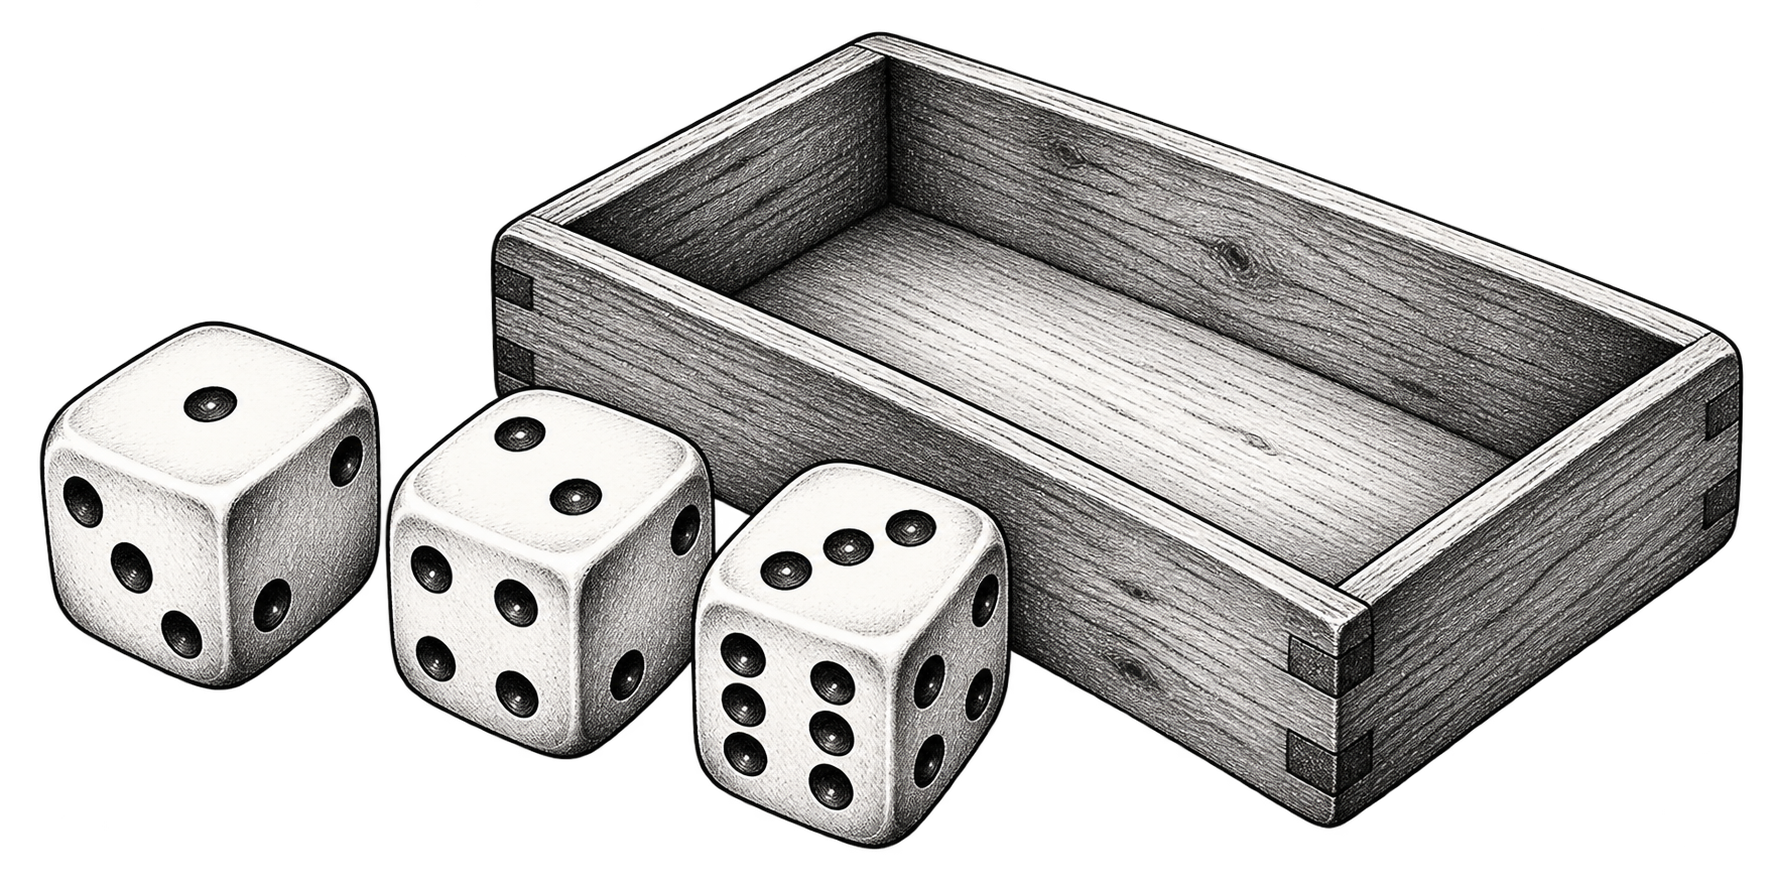
\includegraphics[width=19cm,height=6.0cm,keepaspectratio]{assets/slides/dice.png}};
\node[anchor=north west,inner sep=0pt,text width=28cm,align=left,text=quiet,font=\fontsize{17}{\dimexpr17pt*6/5\relax}\selectfont] at (1.5,1.45) {Think on your own first. Then compare your reasoning with a partner.};
\end{scope}\end{tikzpicture}
\end{frame}

\begin{frame}[plain,fragile]\begin{tikzpicture}[remember picture,overlay,x=1cm,y=1cm]\begin{scope}[shift={(current page.south west)}]
\node[anchor=north west,inner sep=0pt,text width=29cm,align=left,text=quiet,font=\fontsize{13}{\dimexpr13pt*6/5\relax}\selectfont] at (1.5,16.9) {\heavy LESSON 2 / L2-02 / ANSWER};
\node[anchor=north west,inner sep=0pt,text width=1cm,align=left,text=quiet,font=\fontsize{11}{\dimexpr11pt*6/5\relax}\selectfont] at (30,0.8) {\insertframenumber};
\node[anchor=north west,inner sep=0pt,text width=29cm,align=left,text=ink,font=\fontsize{34}{\dimexpr34pt*6/5\relax}\selectfont] at (1.5,15.4) {\heavy A total of three};
\node(body)[anchor=north west,inner sep=0pt,text width=29cm,align=left,text=ink,font=\fontsize{25}{\dimexpr25pt*6/5\relax}\selectfont] at (1.5,12.4) {The four sequences are [3], [1, 2], [2, 1] and [1, 1, 1]. A sequence containing 4, 5 or 6 already exceeds the target. We count valid sequences rather than simulate random throws.};
\node[anchor=north west,inner sep=0pt,text width=28cm,align=left,text=teal,font=\fontsize{21}{\dimexpr21pt*6/5\relax}\selectfont] at (1.5,4.0) {\textbf{Watch for:} Unordered partitions count [1, 2] only once and solve a different problem.};
\end{scope}\end{tikzpicture}
\end{frame}

\begin{frame}[plain,fragile]\begin{tikzpicture}[remember picture,overlay,x=1cm,y=1cm]\begin{scope}[shift={(current page.south west)}]
\node[anchor=north west,inner sep=0pt,text width=29cm,align=left,text=quiet,font=\fontsize{13}{\dimexpr13pt*6/5\relax}\selectfont] at (1.5,16.9) {\heavy LESSON 2 / L2-03 / QUESTION};
\node[anchor=north west,inner sep=0pt,text width=1cm,align=left,text=quiet,font=\fontsize{11}{\dimexpr11pt*6/5\relax}\selectfont] at (30,0.8) {\insertframenumber};
\node[anchor=north west,inner sep=0pt,text width=29cm,align=left,text=ink,font=\fontsize{34}{\dimexpr34pt*6/5\relax}\selectfont] at (1.5,15.4) {\heavy Six possible last numbers};
\node(body)[anchor=north west,inner sep=0pt,text width=29cm,align=left,text=ink,font=\fontsize{22}{\dimexpr22pt*6/5\relax}\selectfont] at (1.5,12.4) {Let ways[total] count ordered sequences of values 1 to 6 whose sum is that total. Explain ways[0] = 1. For target 4, group sequences by their last number and add the earlier counts. Copy your L2-02 count into total 3, then fill totals 5, 6 and 7 in the table.};
\node(tab)[anchor=north west,inner sep=0,text width=29cm] at ([yshift=-8mm]body.south west) {\begingroup\fontsize{22}{26}\selectfont\setlength{\tabcolsep}{5pt}\setlength{\arrayrulewidth}{.5pt}\arrayrulecolor{quiet}\renewcommand{\arraystretch}{1}\begin{tabularx}{\linewidth}{|>{\raggedright\arraybackslash}p{57mm}|>{\centering\arraybackslash}X|>{\centering\arraybackslash}X|>{\centering\arraybackslash}X|>{\centering\arraybackslash}X|>{\centering\arraybackslash}X|>{\centering\arraybackslash}X|>{\centering\arraybackslash}X|>{\centering\arraybackslash}X|}\hline
\rowcolor{wash}\rule[-3mm]{0pt}{9.5mm}\textbf{Total} & \textbf{0} & \textbf{1} & \textbf{2} & \textbf{3} & \textbf{4} & \textbf{5} & \textbf{6} & \textbf{7}\\\hline
\rule[-4.6mm]{0pt}{13.5mm}ways[total] & 1 & 1 & 2 &  &  &  &  & \\\hline
\end{tabularx}\endgroup};
\end{scope}\end{tikzpicture}
\end{frame}

\begin{frame}[plain,fragile]\begin{tikzpicture}[remember picture,overlay,x=1cm,y=1cm]\begin{scope}[shift={(current page.south west)}]
\node[anchor=north west,inner sep=0pt,text width=29cm,align=left,text=quiet,font=\fontsize{13}{\dimexpr13pt*6/5\relax}\selectfont] at (1.5,16.9) {\heavy LESSON 2 / L2-03 / ANSWER};
\node[anchor=north west,inner sep=0pt,text width=1cm,align=left,text=quiet,font=\fontsize{11}{\dimexpr11pt*6/5\relax}\selectfont] at (30,0.8) {\insertframenumber};
\node[anchor=north west,inner sep=0pt,text width=29cm,align=left,text=ink,font=\fontsize{34}{\dimexpr34pt*6/5\relax}\selectfont] at (1.5,15.4) {\heavy Six possible last numbers};
\node(body)[anchor=north west,inner sep=0pt,text width=29cm,align=left,text=ink,font=\fontsize{22}{\dimexpr22pt*6/5\relax}\selectfont] at (1.5,12.4) {The empty sequence is the one sequence with total 0. For total 4, final numbers 1, 2, 3 and 4 give counts 4 + 2 + 1 + 1 = 8. Totals 5 and 6 give 16 and 32. Total 7 uses totals 6 through 1: 32 + 16 + 8 + 4 + 2 + 1 = 63.};
\node(tab)[anchor=north west,inner sep=0,text width=29cm] at ([yshift=-8mm]body.south west) {\begingroup\fontsize{22}{26}\selectfont\setlength{\tabcolsep}{5pt}\setlength{\arrayrulewidth}{.5pt}\arrayrulecolor{quiet}\renewcommand{\arraystretch}{1}\begin{tabularx}{\linewidth}{|>{\raggedright\arraybackslash}p{57mm}|>{\centering\arraybackslash}X|>{\centering\arraybackslash}X|>{\centering\arraybackslash}X|>{\centering\arraybackslash}X|>{\centering\arraybackslash}X|>{\centering\arraybackslash}X|>{\centering\arraybackslash}X|>{\centering\arraybackslash}X|}\hline
\rowcolor{wash}\rule[-3mm]{0pt}{9.5mm}\textbf{Total} & \textbf{0} & \textbf{1} & \textbf{2} & \textbf{3} & \textbf{4} & \textbf{5} & \textbf{6} & \textbf{7}\\\hline
\rule[-4.6mm]{0pt}{13.5mm}ways[total] & 1 & 1 & 2 & 4 & 8 & 16 & 32 & 63\\\hline
\end{tabularx}\endgroup};
\end{scope}\end{tikzpicture}
\end{frame}

\begin{frame}[plain,fragile]\begin{tikzpicture}[remember picture,overlay,x=1cm,y=1cm]\begin{scope}[shift={(current page.south west)}]
\node[anchor=north west,inner sep=0pt,text width=29cm,align=left,text=quiet,font=\fontsize{13}{\dimexpr13pt*6/5\relax}\selectfont] at (1.5,16.9) {\heavy LESSON 2 / L2-04 / QUESTION};
\node[anchor=north west,inner sep=0pt,text width=1cm,align=left,text=quiet,font=\fontsize{11}{\dimexpr11pt*6/5\relax}\selectfont] at (30,0.8) {\insertframenumber};
\node[anchor=north west,inner sep=0pt,text width=29cm,align=left,text=ink,font=\fontsize{34}{\dimexpr34pt*6/5\relax}\selectfont] at (1.5,15.4) {\heavy Dice: recursion, then caching};
\node(body)[anchor=north west,inner sep=0pt,text width=29cm,align=left,text=ink,font=\fontsize{20}{\dimexpr20pt*6/5\relax}\selectfont] at (1.5,12.4) {Write dice\_slow(n) recursively to count ordered sequences of faces 1 to 6 with total n. Trace target 4. Then write dice\_cached(n), adding a cache: which input identifies a repeated question? Use the uncached version only on tiny targets. In the cached version, store counts modulo 1,000,000,007.};
\node(sig)[anchor=north west,inner sep=3mm,fill=codepaper,align=left,font=\ttfamily\fontsize{16}{20}\selectfont] at ([yshift=-4mm,xshift=3mm]body.south west) {def dice\_slow(n):\\\hspace*{2.4em}return None  \# Replace this\\def dice\_cached(n):\\\hspace*{2.4em}def count(total):\\\hspace*{4.8em}return None  \# Replace this\\\hspace*{2.4em}return count(n)};
\node(result)[anchor=north west,inner sep=0pt,text width=13.5cm,align=left,text=quiet,font=\fontsize{17}{20}\selectfont] at ([yshift=-4mm,xshift=15.5cm]body.south west) {\textbf{Returns}\par \textbf{dice\_slow(n)}: the exact number of ordered dice sequences with total n.\par\smallskip \textbf{dice\_cached(n)}: the count for total n, modulo 1,000,000,007.\par\smallskip \textbf{count(total)}: the count for this total, modulo 1,000,000,007.\par\smallskip };
\node(both)[fit=(sig)(result),inner sep=0] {};
\node[anchor=north west,inner sep=0pt,text width=29cm,align=left,text=quiet,font=\fontsize{18}{22}\selectfont] at ([yshift=-3mm,xshift=-3mm]both.south west) {\textbf{Hints.} What is the count for total 0? Which faces can be the last one when the remaining total is small? What input identifies a repeated question, and where must the saved answers live so that every call shares them?};
\end{scope}\end{tikzpicture}
\end{frame}

\begin{frame}[plain,fragile]\begin{tikzpicture}[remember picture,overlay,x=1cm,y=1cm]\begin{scope}[shift={(current page.south west)}]
\node[anchor=north west,inner sep=0pt,text width=29cm,align=left,text=quiet,font=\fontsize{13}{\dimexpr13pt*6/5\relax}\selectfont] at (1.5,16.9) {\heavy LESSON 2 / L2-04 / ANSWER};
\node[anchor=north west,inner sep=0pt,text width=1cm,align=left,text=quiet,font=\fontsize{11}{\dimexpr11pt*6/5\relax}\selectfont] at (30,0.8) {\insertframenumber};
\node[anchor=north west,inner sep=0pt,text width=29cm,align=left,text=ink,font=\fontsize{34}{\dimexpr34pt*6/5\relax}\selectfont] at (1.5,15.4) {\heavy Dice: recursion, then caching};
\node(body)[anchor=north west,inner sep=0pt,text width=29cm,align=left,text=ink,font=\fontsize{25}{\dimexpr25pt*6/5\relax}\selectfont] at (1.5,12.4) {Use one cache key per target total. Total 0 contributes 1. For a positive total, try each final face that fits and add the counts for the smaller targets. Faces larger than the remaining total are skipped, so no negative total is ever asked. Target 4 returns 8. A repeated target reads its saved answer instead of branching again.};
\node[anchor=north west,inner sep=0pt,text width=28cm,align=left,text=teal,font=\fontsize{21}{\dimexpr21pt*6/5\relax}\selectfont] at (1.5,4.0) {\textbf{Watch for:} Caching is valid because the allowed faces remain fixed throughout one call.};
\end{scope}\end{tikzpicture}
\end{frame}

\begin{frame}[plain,fragile]
\begin{lrbox}{\codebox}\begin{minipage}{794pt}
\begin{lstlisting}[basicstyle=\ttfamily\fontsize{18.0}{20.2}\selectfont\color{ink},numbers=left,numberstyle=\ttfamily\fontsize{11.7}{20.2}\selectfont\color{quiet},numbersep=12pt,xleftmargin=21pt,firstnumber=1,breaklines=false,aboveskip=0pt,belowskip=0pt]
def dice_slow(n):
    if n == 0:
        return 1
    return sum(dice_slow(n - face) for face in range(1, min(6, n) + 1))
\end{lstlisting}
\end{minipage}\end{lrbox}
\begin{tikzpicture}[remember picture,overlay,x=1cm,y=1cm]\begin{scope}[shift={(current page.south west)}]
\node[anchor=north west,inner sep=0pt,text width=29cm,align=left,text=quiet,font=\fontsize{13}{\dimexpr13pt*6/5\relax}\selectfont] at (1.5,16.9) {\heavy LESSON 2 / L2-04 / ANSWER: PYTHON};
\node[anchor=north west,inner sep=0pt,text width=1cm,align=left,text=quiet,font=\fontsize{11}{\dimexpr11pt*6/5\relax}\selectfont] at (30,0.8) {\insertframenumber};
\node[anchor=north west,inner sep=0pt,text width=29cm,align=left,text=ink,font=\fontsize{34}{40.8}\selectfont] at (1.5,15.4) {\heavy dice slow};
\node[anchor=north,inner sep=5mm,fill=codepaper] at (16,13.6) {\usebox{\codebox}};
\end{scope}\end{tikzpicture}

\end{frame}

\begin{frame}[plain,fragile]
\begin{lrbox}{\codebox}\begin{minipage}{799pt}
\begin{lstlisting}[basicstyle=\ttfamily\fontsize{20.5}{23.0}\selectfont\color{ink},numbers=left,numberstyle=\ttfamily\fontsize{13.3}{23.0}\selectfont\color{quiet},numbersep=12pt,xleftmargin=30pt,firstnumber=1,breaklines=false,aboveskip=0pt,belowskip=0pt]
MOD = 1_000_000_007

def dice_cached(n):
    cache = {0: 1}
    def count(total):
        if total not in cache:
            cache[total] = sum(count(total - face)
                for face in range(1, min(6, total) + 1)) % MOD
        return cache[total]
    return count(n)
\end{lstlisting}
\end{minipage}\end{lrbox}
\begin{tikzpicture}[remember picture,overlay,x=1cm,y=1cm]\begin{scope}[shift={(current page.south west)}]
\node[anchor=north west,inner sep=0pt,text width=29cm,align=left,text=quiet,font=\fontsize{13}{\dimexpr13pt*6/5\relax}\selectfont] at (1.5,16.9) {\heavy LESSON 2 / L2-04 / ANSWER: PYTHON};
\node[anchor=north west,inner sep=0pt,text width=1cm,align=left,text=quiet,font=\fontsize{11}{\dimexpr11pt*6/5\relax}\selectfont] at (30,0.8) {\insertframenumber};
\node[anchor=north west,inner sep=0pt,text width=29cm,align=left,text=ink,font=\fontsize{34}{40.8}\selectfont] at (1.5,15.4) {\heavy dice cached};
\node[anchor=north,inner sep=5mm,fill=codepaper] at (16,13.6) {\usebox{\codebox}};
\end{scope}\end{tikzpicture}

\end{frame}

\begin{frame}[plain,fragile]\begin{tikzpicture}[remember picture,overlay,x=1cm,y=1cm]\begin{scope}[shift={(current page.south west)}]
\node[anchor=north west,inner sep=0pt,text width=29cm,align=left,text=quiet,font=\fontsize{13}{\dimexpr13pt*6/5\relax}\selectfont] at (1.5,16.9) {\heavy LESSON 2 / L2-05 / QUESTION};
\node[anchor=north west,inner sep=0pt,text width=1cm,align=left,text=quiet,font=\fontsize{11}{\dimexpr11pt*6/5\relax}\selectfont] at (30,0.8) {\insertframenumber};
\node[anchor=north west,inner sep=0pt,text width=29cm,align=left,text=ink,font=\fontsize{34}{\dimexpr34pt*6/5\relax}\selectfont] at (1.5,15.4) {\heavy Dice: fill the totals in order};
\node(body)[anchor=north west,inner sep=0pt,text width=29cm,align=left,text=ink,font=\fontsize{20}{\dimexpr20pt*6/5\relax}\selectfont] at (1.5,12.4) {Write dice\_table(n) using a loop. Store in ways[total] the count for that total, modulo 1,000,000,007. Fill totals from 1 upwards. When the loop reaches total 7, which earlier totals does it read? Add their counts and explain the result.};
\node(sig)[anchor=north west,inner sep=3mm,fill=codepaper,align=left,font=\ttfamily\fontsize{16}{20}\selectfont] at ([yshift=-4mm,xshift=3mm]body.south west) {def dice\_table(n):\\\hspace*{2.4em}return None  \# Replace this};
\node(result)[anchor=north west,inner sep=0pt,text width=13.5cm,align=left,text=quiet,font=\fontsize{17}{20}\selectfont] at ([yshift=-4mm,xshift=15.5cm]body.south west) {\textbf{Returns}\par \textbf{dice\_table(n)}: the number of ordered dice sequences with total n, modulo 1,000,000,007.\par\smallskip };
\node(both)[fit=(sig)(result),inner sep=0] {};
\node[anchor=north west,inner sep=0pt,text width=29cm,align=left,text=quiet,font=\fontsize{18}{22}\selectfont] at ([yshift=-3mm,xshift=-3mm]both.south west) {\textbf{Hints.} Which entry is known before the loop? For each total, which earlier totals can the last face come from? Where do you take the remainder so that stored numbers stay small?};
\end{scope}\end{tikzpicture}
\end{frame}

\begin{frame}[plain,fragile]\begin{tikzpicture}[remember picture,overlay,x=1cm,y=1cm]\begin{scope}[shift={(current page.south west)}]
\node[anchor=north west,inner sep=0pt,text width=29cm,align=left,text=quiet,font=\fontsize{13}{\dimexpr13pt*6/5\relax}\selectfont] at (1.5,16.9) {\heavy LESSON 2 / L2-05 / ANSWER};
\node[anchor=north west,inner sep=0pt,text width=1cm,align=left,text=quiet,font=\fontsize{11}{\dimexpr11pt*6/5\relax}\selectfont] at (30,0.8) {\insertframenumber};
\node[anchor=north west,inner sep=0pt,text width=29cm,align=left,text=ink,font=\fontsize{34}{\dimexpr34pt*6/5\relax}\selectfont] at (1.5,15.4) {\heavy Dice: fill the totals in order};
\node(body)[anchor=north west,inner sep=0pt,text width=29cm,align=left,text=ink,font=\fontsize{25}{\dimexpr25pt*6/5\relax}\selectfont] at (1.5,12.4) {Total 7 reads counts for totals 6, 5, 4, 3, 2 and 1. Their sum is 32 + 16 + 8 + 4 + 2 + 1 = 63. Fill totals from 1 upwards, starting with ways[0] = 1.};
\node[anchor=north west,inner sep=0pt,text width=28cm,align=left,text=teal,font=\fontsize{21}{\dimexpr21pt*6/5\relax}\selectfont] at (1.5,4.0) {\textbf{Watch for:} Do not fill a list with zeros and forget the one empty sequence.};
\end{scope}\end{tikzpicture}
\end{frame}

\begin{frame}[plain,fragile]
\begin{lrbox}{\codebox}\begin{minipage}{744pt}
\begin{lstlisting}[basicstyle=\ttfamily\fontsize{24.0}{26.9}\selectfont\color{ink},numbers=left,numberstyle=\ttfamily\fontsize{15.6}{26.9}\selectfont\color{quiet},numbersep=12pt,xleftmargin=33pt,firstnumber=1,breaklines=false,aboveskip=0pt,belowskip=0pt]
MOD = 1_000_000_007

def dice_table(n):
    ways = [0] * (n + 1)
    ways[0] = 1
    for total in range(1, n + 1):
        for face in range(1, 7):
            if total >= face:
                ways[total] += ways[total - face]
        ways[total] %= MOD
    return ways[n]
\end{lstlisting}
\end{minipage}\end{lrbox}
\begin{tikzpicture}[remember picture,overlay,x=1cm,y=1cm]\begin{scope}[shift={(current page.south west)}]
\node[anchor=north west,inner sep=0pt,text width=29cm,align=left,text=quiet,font=\fontsize{13}{\dimexpr13pt*6/5\relax}\selectfont] at (1.5,16.9) {\heavy LESSON 2 / L2-05 / ANSWER: PYTHON};
\node[anchor=north west,inner sep=0pt,text width=1cm,align=left,text=quiet,font=\fontsize{11}{\dimexpr11pt*6/5\relax}\selectfont] at (30,0.8) {\insertframenumber};
\node[anchor=north west,inner sep=0pt,text width=29cm,align=left,text=ink,font=\fontsize{34}{40.8}\selectfont] at (1.5,15.4) {\heavy dice table};
\node[anchor=north,inner sep=5mm,fill=codepaper] at (16,13.6) {\usebox{\codebox}};
\end{scope}\end{tikzpicture}

\end{frame}

\begin{frame}[plain,fragile]\begin{tikzpicture}[remember picture,overlay,x=1cm,y=1cm]\begin{scope}[shift={(current page.south west)}]
\node[anchor=north west,inner sep=0pt,text width=29cm,align=left,text=quiet,font=\fontsize{13}{\dimexpr13pt*6/5\relax}\selectfont] at (1.5,16.9) {\heavy LESSON 2 / L2-06 / QUESTION};
\node[anchor=north west,inner sep=0pt,text width=1cm,align=left,text=quiet,font=\fontsize{11}{\dimexpr11pt*6/5\relax}\selectfont] at (30,0.8) {\insertframenumber};
\node[anchor=north west,inner sep=0pt,text width=29cm,align=left,text=ink,font=\fontsize{34}{\dimexpr34pt*6/5\relax}\selectfont] at (1.5,15.4) {\heavy Why take a remainder?};
\node(body)[anchor=north west,inner sep=0pt,text width=29cm,align=left,text=ink,font=\fontsize{25}{\dimexpr25pt*6/5\relax}\selectfont] at (1.5,12.4) {Modulo 7 means the remainder after division by 7. Compare (12 + 13) \% 7 with ((12 \% 7) + (13 \% 7)) \% 7. Why do both calculations give the same remainder? How does this help when dice counts become very large?};
\node[anchor=north west,inner sep=0pt,text width=28cm,align=left,text=teal,font=\fontsize{22}{\dimexpr22pt*6/5\relax}\selectfont] at (1.5,4.0) {Think on your own first. Then compare your reasoning with a partner.};
\end{scope}\end{tikzpicture}
\end{frame}

\begin{frame}[plain,fragile]
\begin{tikzpicture}[remember picture,overlay,x=1cm,y=1cm]\begin{scope}[shift={(current page.south west)}]
\node[anchor=north west,inner sep=0pt,text width=29cm,align=left,text=quiet,font=\fontsize{13}{\dimexpr13pt*6/5\relax}\selectfont] at (1.5,16.9) {\heavy LESSON 2 / L2-06 / ANSWER};
\node[anchor=north west,inner sep=0pt,text width=1cm,align=left,text=quiet,font=\fontsize{11}{\dimexpr11pt*6/5\relax}\selectfont] at (30,0.8) {\insertframenumber};
\node[anchor=north west,inner sep=0pt,text width=29cm,align=left,text=ink,font=\fontsize{34}{\dimexpr34pt*6/5\relax}\selectfont] at (1.5,15.4) {\heavy Why take a remainder?};
\node(body)[anchor=north west,inner sep=0pt,text width=29cm,align=left,text=ink,font=\fontsize{25}{\dimexpr25pt*6/5\relax}\selectfont] at (1.5,12.4) {12 + 13 = 25, whose remainder is 4. Separately, 12 has remainder 5 and 13 has remainder 6; 5 + 6 = 11 also has remainder 4. Removing whole multiples of 7 does not change a remainder modulo 7. Dice uses the same rule with 1,000,000,007 to keep stored numbers small.};
\node[anchor=north west,inner sep=0pt,text width=28cm,align=left,text=teal,font=\fontsize{21}{\dimexpr21pt*6/5\relax}\selectfont] at (1.5,4.0) {\textbf{Watch for:} The modulo operation is not a probability and does not count only a subset of sequences.};
\end{scope}\end{tikzpicture}
\end{frame}

\begin{frame}[plain,fragile]\begin{tikzpicture}[remember picture,overlay,x=1cm,y=1cm]\begin{scope}[shift={(current page.south west)}]
\node[anchor=north west,inner sep=0pt,text width=29cm,align=left,text=quiet,font=\fontsize{13}{\dimexpr13pt*6/5\relax}\selectfont] at (1.5,16.9) {\heavy LESSON 2 / L2-07 / QUESTION};
\node[anchor=north west,inner sep=0pt,text width=1cm,align=left,text=quiet,font=\fontsize{11}{\dimexpr11pt*6/5\relax}\selectfont] at (30,0.8) {\insertframenumber};
\node[anchor=north west,inner sep=0pt,text width=29cm,align=left,text=ink,font=\fontsize{34}{\dimexpr34pt*6/5\relax}\selectfont] at (1.5,15.4) {\heavy Your turn: three faces};
\node(body)[anchor=north west,inner sep=0pt,text width=29cm,align=left,text=ink,font=\fontsize{20}{\dimexpr20pt*6/5\relax}\selectfont] at (1.5,12.4) {Write dice\_123(n) by adapting dice\_table from L2-05 to allow only faces 1, 2 and 3. First fill counts for totals 0 through 5, then write and test your code. Explain the answer for total 5.};
\node(tab)[anchor=north west,inner sep=0,text width=29cm] at ([yshift=-8mm]body.south west) {\begingroup\fontsize{18}{22}\selectfont\setlength{\tabcolsep}{5pt}\setlength{\arrayrulewidth}{.5pt}\arrayrulecolor{quiet}\renewcommand{\arraystretch}{1}\begin{tabularx}{\linewidth}{|>{\raggedright\arraybackslash}p{57mm}|>{\centering\arraybackslash}X|>{\centering\arraybackslash}X|>{\centering\arraybackslash}X|>{\centering\arraybackslash}X|>{\centering\arraybackslash}X|>{\centering\arraybackslash}X|}\hline
\rowcolor{wash}\rule[-2.6mm]{0pt}{8mm}\textbf{Total} & \textbf{0} & \textbf{1} & \textbf{2} & \textbf{3} & \textbf{4} & \textbf{5}\\\hline
\rule[-3.4mm]{0pt}{8.5mm}ways[total] & 1 &  &  &  &  & \\\hline
\end{tabularx}\endgroup};
\node(sig)[anchor=north west,inner sep=3mm,fill=codepaper,align=left,font=\ttfamily\fontsize{16}{20}\selectfont] at ([yshift=-4mm,xshift=3mm]tab.south west) {def dice\_123(n):\\\hspace*{2.4em}return None  \# Replace this};
\node(result)[anchor=north west,inner sep=0pt,text width=13.5cm,align=left,text=quiet,font=\fontsize{17}{20}\selectfont] at ([yshift=-4mm,xshift=15.5cm]tab.south west) {\textbf{Returns}\par \textbf{dice\_123(n)}: the number of ordered sequences of 1, 2 and 3 with total n, modulo 1,000,000,007.\par\smallskip };
\node(both)[fit=(sig)(result),inner sep=0] {};
\node[anchor=north west,inner sep=0pt,text width=29cm,align=left,text=quiet,font=\fontsize{18}{22}\selectfont] at ([yshift=-3mm,xshift=-3mm]both.south west) {\textbf{Hints.} Which part of dice\_table depends on the faces allowed? Check total 4 by hand before you run the code.};
\end{scope}\end{tikzpicture}
\end{frame}

\begin{frame}[plain,fragile]\begin{tikzpicture}[remember picture,overlay,x=1cm,y=1cm]\begin{scope}[shift={(current page.south west)}]
\node[anchor=north west,inner sep=0pt,text width=29cm,align=left,text=quiet,font=\fontsize{13}{\dimexpr13pt*6/5\relax}\selectfont] at (1.5,16.9) {\heavy LESSON 2 / L2-07 / ANSWER};
\node[anchor=north west,inner sep=0pt,text width=1cm,align=left,text=quiet,font=\fontsize{11}{\dimexpr11pt*6/5\relax}\selectfont] at (30,0.8) {\insertframenumber};
\node[anchor=north west,inner sep=0pt,text width=29cm,align=left,text=ink,font=\fontsize{34}{\dimexpr34pt*6/5\relax}\selectfont] at (1.5,15.4) {\heavy Your turn: three faces};
\node(body)[anchor=north west,inner sep=0pt,text width=29cm,align=left,text=ink,font=\fontsize{22}{\dimexpr22pt*6/5\relax}\selectfont] at (1.5,12.4) {The counts are [1, 1, 2, 4, 7, 13]. Total 5 combines totals 4, 3 and 2, giving 7 + 4 + 2 = 13. Only the allowed-face loop changes.};
\node(tab)[anchor=north west,inner sep=0,text width=29cm] at ([yshift=-8mm]body.south west) {\begingroup\fontsize{22}{26}\selectfont\setlength{\tabcolsep}{5pt}\setlength{\arrayrulewidth}{.5pt}\arrayrulecolor{quiet}\renewcommand{\arraystretch}{1}\begin{tabularx}{\linewidth}{|>{\raggedright\arraybackslash}p{57mm}|>{\centering\arraybackslash}X|>{\centering\arraybackslash}X|>{\centering\arraybackslash}X|>{\centering\arraybackslash}X|>{\centering\arraybackslash}X|>{\centering\arraybackslash}X|}\hline
\rowcolor{wash}\rule[-3mm]{0pt}{9.5mm}\textbf{Total} & \textbf{0} & \textbf{1} & \textbf{2} & \textbf{3} & \textbf{4} & \textbf{5}\\\hline
\rule[-4.6mm]{0pt}{13.5mm}ways[total] & 1 & 1 & 2 & 4 & 7 & 13\\\hline
\end{tabularx}\endgroup};
\end{scope}\end{tikzpicture}
\end{frame}

\begin{frame}[plain,fragile]
\begin{lrbox}{\codebox}\begin{minipage}{744pt}
\begin{lstlisting}[basicstyle=\ttfamily\fontsize{24.0}{26.9}\selectfont\color{ink},numbers=left,numberstyle=\ttfamily\fontsize{15.6}{26.9}\selectfont\color{quiet},numbersep=12pt,xleftmargin=33pt,firstnumber=1,breaklines=false,aboveskip=0pt,belowskip=0pt]
MOD = 1_000_000_007

def dice_123(n):
    ways = [0] * (n + 1)
    ways[0] = 1
    for total in range(1, n + 1):
        for face in (1, 2, 3):
            if total >= face:
                ways[total] += ways[total - face]
        ways[total] %= MOD
    return ways[n]
\end{lstlisting}
\end{minipage}\end{lrbox}
\begin{tikzpicture}[remember picture,overlay,x=1cm,y=1cm]\begin{scope}[shift={(current page.south west)}]
\node[anchor=north west,inner sep=0pt,text width=29cm,align=left,text=quiet,font=\fontsize{13}{\dimexpr13pt*6/5\relax}\selectfont] at (1.5,16.9) {\heavy LESSON 2 / L2-07 / ANSWER: PYTHON};
\node[anchor=north west,inner sep=0pt,text width=1cm,align=left,text=quiet,font=\fontsize{11}{\dimexpr11pt*6/5\relax}\selectfont] at (30,0.8) {\insertframenumber};
\node[anchor=north west,inner sep=0pt,text width=29cm,align=left,text=ink,font=\fontsize{34}{40.8}\selectfont] at (1.5,15.4) {\heavy dice 123};
\node[anchor=north,inner sep=5mm,fill=codepaper] at (16,13.6) {\usebox{\codebox}};
\end{scope}\end{tikzpicture}

\end{frame}

\begin{frame}[plain,fragile]\begin{tikzpicture}[remember picture,overlay,x=1cm,y=1cm]\begin{scope}[shift={(current page.south west)}]
\node[anchor=north west,inner sep=0pt,text width=29cm,align=left,text=quiet,font=\fontsize{13}{\dimexpr13pt*6/5\relax}\selectfont] at (1.5,16.9) {\heavy LESSON 2 / L2-08 / BUFFER / QUESTION};
\node[anchor=north west,inner sep=0pt,text width=1cm,align=left,text=quiet,font=\fontsize{11}{\dimexpr11pt*6/5\relax}\selectfont] at (30,0.8) {\insertframenumber};
\node[anchor=north west,inner sep=0pt,text width=29cm,align=left,text=ink,font=\fontsize{34}{\dimexpr34pt*6/5\relax}\selectfont] at (1.5,15.4) {\heavy Which earlier answers can we forget?};
\node(body)[anchor=north west,inner sep=0pt,text width=29cm,align=left,text=ink,font=\fontsize{24}{\dimexpr24pt*6/5\relax}\selectfont] at (1.5,12.4) {To count sequences for total 7, the last face is 1 to 6. Which earlier totals do we read? For total 8, which count stops being needed?};
\end{scope}\end{tikzpicture}
\end{frame}

\begin{frame}[plain,fragile]\begin{tikzpicture}[remember picture,overlay,x=1cm,y=1cm]\begin{scope}[shift={(current page.south west)}]
\node[anchor=north west,inner sep=0pt,text width=29cm,align=left,text=quiet,font=\fontsize{13}{\dimexpr13pt*6/5\relax}\selectfont] at (1.5,16.9) {\heavy LESSON 2 / L2-08 / BUFFER / ANSWER};
\node[anchor=north west,inner sep=0pt,text width=1cm,align=left,text=quiet,font=\fontsize{11}{\dimexpr11pt*6/5\relax}\selectfont] at (30,0.8) {\insertframenumber};
\node[anchor=north west,inner sep=0pt,text width=29cm,align=left,text=ink,font=\fontsize{34}{\dimexpr34pt*6/5\relax}\selectfont] at (1.5,15.4) {\heavy Only six earlier counts are needed};
\node(body)[anchor=north west,inner sep=0pt,text width=29cm,align=left,text=ink,font=\fontsize{24}{\dimexpr24pt*6/5\relax}\selectfont] at (1.5,12.4) {Total 7 reads counts for totals 1 to 6. Total 8 reads totals 2 to 7. After computing total 7, the count for total 1 can be overwritten. Six reused entries give O(1) memory; we still compute n answers, taking O(n) time.};
\node[anchor=north west,inner sep=0,text width=29cm] at ([yshift=-8mm]body.south west) {\begingroup\fontsize{22}{26}\selectfont\setlength{\tabcolsep}{5pt}\setlength{\arrayrulewidth}{.5pt}\arrayrulecolor{quiet}\renewcommand{\arraystretch}{1}\begin{tabularx}{\linewidth}{|>{\raggedright\arraybackslash}p{52mm}|>{\centering\arraybackslash}X|>{\centering\arraybackslash}X|>{\centering\arraybackslash}X|}\hline
\rowcolor{wash}\rule[-3mm]{0pt}{9.5mm}\textbf{Next total} & \textbf{Reads totals} & \textbf{Counts added} & \textbf{Answer}\\\hline
\rule[-4.6mm]{0pt}{13.5mm}7 & 1 to 6 & 1 + 2 + 4 + 8 + 16 + 32 & 63\\\hline
\rule[-4.6mm]{0pt}{13.5mm}8 & 2 to 7 & 2 + 4 + 8 + 16 + 32 + 63 & 125\\\hline
\end{tabularx}\endgroup};
\end{scope}\end{tikzpicture}
\end{frame}

\begin{frame}[plain,fragile]\begin{tikzpicture}[remember picture,overlay,x=1cm,y=1cm]\begin{scope}[shift={(current page.south west)}]
\node[anchor=north west,inner sep=0pt,text width=29cm,align=left,text=quiet,font=\fontsize{13}{\dimexpr13pt*6/5\relax}\selectfont] at (1.5,16.9) {\heavy LESSON 2 / L2-08 / BUFFER / QUESTION};
\node[anchor=north west,inner sep=0pt,text width=1cm,align=left,text=quiet,font=\fontsize{11}{\dimexpr11pt*6/5\relax}\selectfont] at (30,0.8) {\insertframenumber};
\node[anchor=north west,inner sep=0pt,text width=29cm,align=left,text=ink,font=\fontsize{34}{\dimexpr34pt*6/5\relax}\selectfont] at (1.5,15.4) {\heavy A total is not a slot};
\node(body)[anchor=north west,inner sep=0pt,text width=29cm,align=left,text=ink,font=\fontsize{24}{\dimexpr24pt*6/5\relax}\selectfont] at (1.5,12.4) {Six slots are numbered 0 to 5. Store a count in slot total \% 6. Which slots do totals 5, 6, 7 and 8 use? What must happen before replacing an old count?};
\end{scope}\end{tikzpicture}
\end{frame}

\begin{frame}[plain,fragile]\begin{tikzpicture}[remember picture,overlay,x=1cm,y=1cm]\begin{scope}[shift={(current page.south west)}]
\node[anchor=north west,inner sep=0pt,text width=29cm,align=left,text=quiet,font=\fontsize{13}{\dimexpr13pt*6/5\relax}\selectfont] at (1.5,16.9) {\heavy LESSON 2 / L2-08 / BUFFER / ANSWER};
\node[anchor=north west,inner sep=0pt,text width=1cm,align=left,text=quiet,font=\fontsize{11}{\dimexpr11pt*6/5\relax}\selectfont] at (30,0.8) {\insertframenumber};
\node[anchor=north west,inner sep=0pt,text width=29cm,align=left,text=ink,font=\fontsize{34}{\dimexpr34pt*6/5\relax}\selectfont] at (1.5,15.4) {\heavy The index wraps; the values stay put};
\node(body)[anchor=north west,inner sep=0pt,text width=29cm,align=left,text=ink,font=\fontsize{24}{\dimexpr24pt*6/5\relax}\selectfont] at (1.5,12.4) {Totals 5, 6, 7 and 8 use slots 5, 0, 1 and 2. Read all six counts to form the current answer before overwriting a slot. The same slot holds different totals at different times.};
\node[anchor=north west,inner sep=0,text width=29cm] at ([yshift=-8mm]body.south west) {\begingroup\fontsize{20}{24}\selectfont\setlength{\tabcolsep}{5pt}\setlength{\arrayrulewidth}{.5pt}\arrayrulecolor{quiet}\renewcommand{\arraystretch}{1}\begin{tabularx}{\linewidth}{|>{\raggedright\arraybackslash}p{34mm}|>{\centering\arraybackslash}X|}\hline
\rowcolor{wash}\rule[-2.6mm]{0pt}{8mm}\textbf{Total} & \textbf{Slot calculation}\\\hline
\rule[-3.4mm]{0pt}{11.5mm}5 & 5 \% 6 = 5\\\hline
\rule[-3.4mm]{0pt}{11.5mm}6 & 6 \% 6 = 0\\\hline
\rule[-3.4mm]{0pt}{11.5mm}7 & 7 \% 6 = 1\\\hline
\rule[-3.4mm]{0pt}{11.5mm}8 & 8 \% 6 = 2\\\hline
\end{tabularx}\endgroup};
\end{scope}\end{tikzpicture}
\end{frame}

\begin{frame}[plain,fragile]\begin{tikzpicture}[remember picture,overlay,x=1cm,y=1cm]\begin{scope}[shift={(current page.south west)}]
\node[anchor=north west,inner sep=0pt,text width=29cm,align=left,text=quiet,font=\fontsize{13}{\dimexpr13pt*6/5\relax}\selectfont] at (1.5,16.9) {\heavy LESSON 2 / L2-08 / QUESTION / OPTIONAL};
\node[anchor=north west,inner sep=0pt,text width=1cm,align=left,text=quiet,font=\fontsize{11}{\dimexpr11pt*6/5\relax}\selectfont] at (30,0.8) {\insertframenumber};
\node[anchor=north west,inner sep=0pt,text width=29cm,align=left,text=ink,font=\fontsize{34}{\dimexpr34pt*6/5\relax}\selectfont] at (1.5,15.4) {\heavy Extension: six slots instead of a full table};
\node(body)[anchor=north west,inner sep=0pt,text width=29cm,align=left,text=ink,font=\fontsize{25}{\dimexpr25pt*6/5\relax}\selectfont] at (1.5,12.4) {Before total 7, recent is [32, 1, 2, 4, 8, 16] in slots 0 to 5. These store counts for totals [6, 1, 2, 3, 4, 5]. The running sum window is 63. Which slot does 7 \% 6 choose, and which old count must be saved before overwriting it? Store the answer for total 7, then prepare the next sum. What should dice\_window(7) return? Explain why six slots are enough.};
\node[anchor=north west,inner sep=0pt,text width=28cm,align=left,text=teal,font=\fontsize{22}{\dimexpr22pt*6/5\relax}\selectfont] at (1.5,4.0) {Think on your own first. Then compare your reasoning with a partner.};
\end{scope}\end{tikzpicture}
\end{frame}

\begin{frame}[plain,fragile]\begin{tikzpicture}[remember picture,overlay,x=1cm,y=1cm]\begin{scope}[shift={(current page.south west)}]
\node[anchor=north west,inner sep=0pt,text width=29cm,align=left,text=quiet,font=\fontsize{13}{\dimexpr13pt*6/5\relax}\selectfont] at (1.5,16.9) {\heavy LESSON 2 / L2-08 / ANSWER};
\node[anchor=north west,inner sep=0pt,text width=1cm,align=left,text=quiet,font=\fontsize{11}{\dimexpr11pt*6/5\relax}\selectfont] at (30,0.8) {\insertframenumber};
\node[anchor=north west,inner sep=0pt,text width=29cm,align=left,text=ink,font=\fontsize{34}{\dimexpr34pt*6/5\relax}\selectfont] at (1.5,15.4) {\heavy Extension: six slots instead of a full table};
\node(body)[anchor=north west,inner sep=0pt,text width=29cm,align=left,text=ink,font=\fontsize{22}{\dimexpr22pt*6/5\relax}\selectfont] at (1.5,12.4) {7 \% 6 chooses slot 1. Save its old count 1, then store 63. Prepare the next sum: 63 - 1 + 63 = 125, for total 8. Return recent[1] = 63. Only the six preceding counts are needed: reusing their slots reduces memory from O(n) to O(1). Time remains O(n).};
\node(tab)[anchor=north west,inner sep=0,text width=29cm] at ([yshift=-8mm]body.south west) {\begingroup\fontsize{20}{24}\selectfont\setlength{\tabcolsep}{5pt}\setlength{\arrayrulewidth}{.5pt}\arrayrulecolor{quiet}\renewcommand{\arraystretch}{1}\begin{tabularx}{\linewidth}{|>{\raggedright\arraybackslash}p{73mm}|>{\centering\arraybackslash}X|>{\centering\arraybackslash}X|>{\centering\arraybackslash}X|>{\centering\arraybackslash}X|>{\centering\arraybackslash}X|>{\centering\arraybackslash}X|}\hline
\rowcolor{wash}\rule[-2.6mm]{0pt}{8mm}\textbf{Slot} & \textbf{0} & \textbf{1} & \textbf{2} & \textbf{3} & \textbf{4} & \textbf{5}\\\hline
\rule[-3.4mm]{0pt}{11.5mm}Total before 7 & 6 & 1 & 2 & 3 & 4 & 5\\\hline
\rule[-3.4mm]{0pt}{11.5mm}Count before 7 & 32 & 1 & 2 & 4 & 8 & 16\\\hline
\rule[-3.4mm]{0pt}{11.5mm}Total after 7 & 6 & 7 & 2 & 3 & 4 & 5\\\hline
\rule[-3.4mm]{0pt}{11.5mm}Count after 7 & 32 & 63 & 2 & 4 & 8 & 16\\\hline
\end{tabularx}\endgroup};
\end{scope}\end{tikzpicture}
\end{frame}

\begin{frame}[plain,fragile]
\begin{lrbox}{\codebox}\begin{minipage}{519pt}
\begin{lstlisting}[basicstyle=\ttfamily\fontsize{24.0}{26.9}\selectfont\color{ink},numbers=left,numberstyle=\ttfamily\fontsize{15.6}{26.9}\selectfont\color{quiet},numbersep=12pt,xleftmargin=23pt,firstnumber=1,breaklines=false,aboveskip=0pt,belowskip=0pt]
MOD = 1_000_000_007

def dice_ring(n):
    recent = [0] * 6
    recent[0] = 1
    for total in range(1, n + 1):
        answer = sum(recent) % MOD
        recent[total % 6] = answer
    return recent[n % 6]
\end{lstlisting}
\end{minipage}\end{lrbox}
\begin{tikzpicture}[remember picture,overlay,x=1cm,y=1cm]\begin{scope}[shift={(current page.south west)}]
\node[anchor=north west,inner sep=0pt,text width=29cm,align=left,text=quiet,font=\fontsize{13}{\dimexpr13pt*6/5\relax}\selectfont] at (1.5,16.9) {\heavy LESSON 2 / L2-08 / ANSWER: PYTHON};
\node[anchor=north west,inner sep=0pt,text width=1cm,align=left,text=quiet,font=\fontsize{11}{\dimexpr11pt*6/5\relax}\selectfont] at (30,0.8) {\insertframenumber};
\node[anchor=north west,inner sep=0pt,text width=29cm,align=left,text=ink,font=\fontsize{34}{40.8}\selectfont] at (1.5,15.4) {\heavy dice ring};
\node[anchor=north,inner sep=5mm,fill=codepaper] at (16,13.6) {\usebox{\codebox}};
\end{scope}\end{tikzpicture}

\end{frame}

\begin{frame}[plain,fragile]
\begin{lrbox}{\codebox}\begin{minipage}{797pt}
\begin{lstlisting}[basicstyle=\ttfamily\fontsize{23.0}{25.8}\selectfont\color{ink},numbers=left,numberstyle=\ttfamily\fontsize{15.0}{25.8}\selectfont\color{quiet},numbersep=12pt,xleftmargin=32pt,firstnumber=1,breaklines=false,aboveskip=0pt,belowskip=0pt]
MOD = 1_000_000_007

def dice_window(n):
    recent = [0] * 6
    recent[0] = 1
    window = 1
    for total in range(1, n + 1):
        slot = total % 6
        oldest = recent[slot]
        recent[slot] = window
        window = (window - oldest + recent[slot]) % MOD
    return recent[n % 6]
\end{lstlisting}
\end{minipage}\end{lrbox}
\begin{tikzpicture}[remember picture,overlay,x=1cm,y=1cm]\begin{scope}[shift={(current page.south west)}]
\node[anchor=north west,inner sep=0pt,text width=29cm,align=left,text=quiet,font=\fontsize{13}{\dimexpr13pt*6/5\relax}\selectfont] at (1.5,16.9) {\heavy LESSON 2 / L2-08 / ANSWER: PYTHON};
\node[anchor=north west,inner sep=0pt,text width=1cm,align=left,text=quiet,font=\fontsize{11}{\dimexpr11pt*6/5\relax}\selectfont] at (30,0.8) {\insertframenumber};
\node[anchor=north west,inner sep=0pt,text width=29cm,align=left,text=ink,font=\fontsize{34}{40.8}\selectfont] at (1.5,15.4) {\heavy dice window};
\node[anchor=north,inner sep=5mm,fill=codepaper] at (16,13.6) {\usebox{\codebox}};
\end{scope}\end{tikzpicture}

\end{frame}

\begin{frame}[plain,fragile]\begin{tikzpicture}[remember picture,overlay,x=1cm,y=1cm]\begin{scope}[shift={(current page.south west)}]
\node[anchor=north west,inner sep=0pt,text width=29cm,align=left,text=quiet,font=\fontsize{13}{\dimexpr13pt*6/5\relax}\selectfont] at (1.5,16.9) {\heavy LESSON 2 / L2-09 / QUESTION};
\node[anchor=north west,inner sep=0pt,text width=1cm,align=left,text=quiet,font=\fontsize{11}{\dimexpr11pt*6/5\relax}\selectfont] at (30,0.8) {\insertframenumber};
\node[anchor=north west,inner sep=0pt,text width=29cm,align=left,text=ink,font=\fontsize{34}{\dimexpr34pt*6/5\relax}\selectfont] at (1.5,15.4) {\heavy Grid Paths: draw before coding};
\node(body)[anchor=north west,inner sep=0pt,text width=29cm,align=left,text=ink,font=\fontsize{23}{\dimexpr23pt*6/5\relax}\selectfont] at (1.5,12.4) {In a 3 by 3 grid, a dot is open and a star is blocked. Start at the top left and finish at the bottom right. Move only one cell right or down. The centre cell is blocked. Draw or list every legal route; how many are there?};
\node[anchor=north west,inner sep=0,text width=14cm] at ([yshift=-8mm]body.south west) {\begingroup\fontsize{22}{26}\selectfont\setlength{\tabcolsep}{5pt}\setlength{\arrayrulewidth}{.5pt}\arrayrulecolor{quiet}\renewcommand{\arraystretch}{1}\begin{tabularx}{\linewidth}{|>{\raggedright\arraybackslash}p{62mm}|>{\centering\arraybackslash}X|>{\centering\arraybackslash}X|>{\centering\arraybackslash}X|}\hline
\rowcolor{wash}\rule[-3mm]{0pt}{9.5mm}\textbf{Row / column} & \textbf{0} & \textbf{1} & \textbf{2}\\\hline
\rule[-4.6mm]{0pt}{13.5mm}0 & . & . & .\\\hline
\rule[-4.6mm]{0pt}{13.5mm}1 & . & * & .\\\hline
\rule[-4.6mm]{0pt}{13.5mm}2 & . & . & .\\\hline
\end{tabularx}\endgroup};
\node[anchor=south,inner sep=0] at (24.5,1.8) {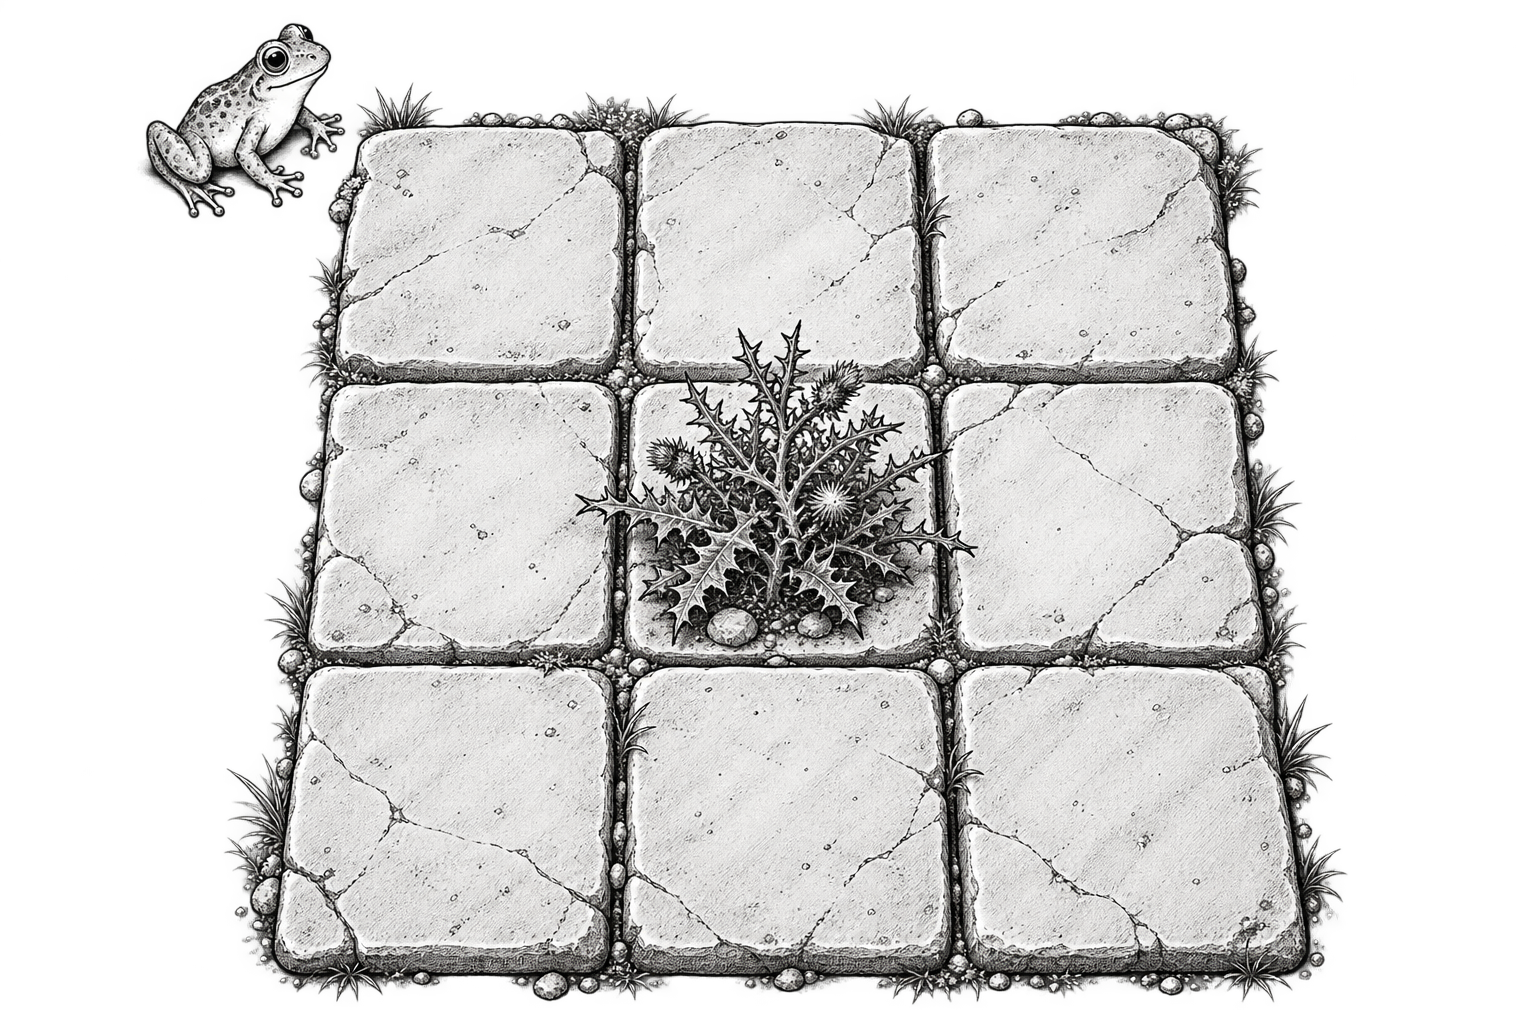
\includegraphics[width=11cm,height=6.8cm,keepaspectratio]{assets/slides/grid.png}};
\end{scope}\end{tikzpicture}
\end{frame}

\begin{frame}[plain,fragile]\begin{tikzpicture}[remember picture,overlay,x=1cm,y=1cm]\begin{scope}[shift={(current page.south west)}]
\node[anchor=north west,inner sep=0pt,text width=29cm,align=left,text=quiet,font=\fontsize{13}{\dimexpr13pt*6/5\relax}\selectfont] at (1.5,16.9) {\heavy LESSON 2 / L2-09 / ANSWER};
\node[anchor=north west,inner sep=0pt,text width=1cm,align=left,text=quiet,font=\fontsize{11}{\dimexpr11pt*6/5\relax}\selectfont] at (30,0.8) {\insertframenumber};
\node[anchor=north west,inner sep=0pt,text width=29cm,align=left,text=ink,font=\fontsize{34}{\dimexpr34pt*6/5\relax}\selectfont] at (1.5,15.4) {\heavy Grid Paths: draw before coding};
\node(body)[anchor=north west,inner sep=0pt,text width=29cm,align=left,text=ink,font=\fontsize{22}{\dimexpr22pt*6/5\relax}\selectfont] at (1.5,12.4) {Two routes remain: right, right, down, down; and down, down, right, right. Every other route would visit the blocked centre square.};
\node[anchor=north west,inner sep=0] at (1.5,9.0) {\scalebox{1.4}{\begin{minipage}{16cm}\begin{center}\begin{tikzpicture}[>=Stealth,every node/.style={font=\fontsize{13}{15}\selectfont},box/.style={draw=teal,rounded corners,minimum width=20mm,minimum height=8mm,fill=wash},arr/.style={->,thick,teal}]\draw[teal,fill=paper] (-0.75,-0.75) rectangle (0.75,0.75);\node[anchor=north west,inner sep=2pt,font=\scriptsize,text=quiet] at (-0.75,0.75) {0,0};\draw[teal,fill=paper] (0.75,-0.75) rectangle (2.25,0.75);\node[anchor=north west,inner sep=2pt,font=\scriptsize,text=quiet] at (0.75,0.75) {0,1};\draw[teal,fill=paper] (2.25,-0.75) rectangle (3.75,0.75);\node[anchor=north west,inner sep=2pt,font=\scriptsize,text=quiet] at (2.25,0.75) {0,2};\draw[teal,fill=paper] (-0.75,-2.25) rectangle (0.75,-0.75);\node[anchor=north west,inner sep=2pt,font=\scriptsize,text=quiet] at (-0.75,-0.75) {1,0};\draw[teal,fill=wash] (0.75,-2.25) rectangle (2.25,-0.75);\node[anchor=north west,inner sep=2pt,font=\scriptsize,text=quiet] at (0.75,-0.75) {1,1};\draw[teal,fill=paper] (2.25,-2.25) rectangle (3.75,-0.75);\node[anchor=north west,inner sep=2pt,font=\scriptsize,text=quiet] at (2.25,-0.75) {1,2};\draw[teal,fill=paper] (-0.75,-3.75) rectangle (0.75,-2.25);\node[anchor=north west,inner sep=2pt,font=\scriptsize,text=quiet] at (-0.75,-2.25) {2,0};\draw[teal,fill=paper] (0.75,-3.75) rectangle (2.25,-2.25);\node[anchor=north west,inner sep=2pt,font=\scriptsize,text=quiet] at (0.75,-2.25) {2,1};\draw[teal,fill=paper] (2.25,-3.75) rectangle (3.75,-2.25);\node[anchor=north west,inner sep=2pt,font=\scriptsize,text=quiet] at (2.25,-2.25) {2,2};\node[font=\Large,text=quiet,inner sep=0pt] at (1.5,-1.4) {*};\node[font=\scriptsize,text=quiet,inner sep=0pt] at (1.5,-1.9) {blocked};\node[anchor=south] at (0,0.75) {start};\node[anchor=north] at (3.0,-3.75) {finish};\draw[arr,line width=1.6pt,shorten >=3pt,shorten <=3pt] (0.0,0.0)--(1.5,0.0);\draw[arr,line width=1.6pt,shorten >=3pt,shorten <=3pt] (1.5,0.0)--(3.0,0.0);\draw[arr,line width=1.6pt,shorten >=3pt,shorten <=3pt] (3.0,0.0)--(3.0,-1.5);\draw[arr,line width=1.6pt,shorten >=3pt,shorten <=3pt] (3.0,-1.5)--(3.0,-3.0);\draw[arr,orange,dashed,line width=1.6pt,shorten >=3pt,shorten <=3pt] (0.0,0.0)--(0.0,-1.5);\draw[arr,orange,dashed,line width=1.6pt,shorten >=3pt,shorten <=3pt] (0.0,-1.5)--(0.0,-3.0);\draw[arr,orange,dashed,line width=1.6pt,shorten >=3pt,shorten <=3pt] (0.0,-3.0)--(1.5,-3.0);\draw[arr,orange,dashed,line width=1.6pt,shorten >=3pt,shorten <=3pt] (1.5,-3.0)--(3.0,-3.0);\fill[teal] (0.0,0.0) circle (3pt);\fill[teal] (3.0,-3.0) circle (3pt);\draw[arr,line width=1.6pt] (4.8,-0.4)--(6.0,-0.4);\node[anchor=west] at (6.1,-0.4) {Route 1: right, right, down, down};\draw[arr,orange,dashed,line width=1.6pt] (4.8,-1.3)--(6.0,-1.3);\node[anchor=west] at (6.1,-1.3) {Route 2: down, down, right, right};\node[anchor=north west,text width=62mm,inner sep=0pt] at (4.8,-2.0) {Every other route enters the blocked centre (1,1). Cells are labelled row, column.};\end{tikzpicture}\end{center}\end{minipage}}};
\end{scope}\end{tikzpicture}
\end{frame}

\begin{frame}[plain,fragile]\begin{tikzpicture}[remember picture,overlay,x=1cm,y=1cm]\begin{scope}[shift={(current page.south west)}]
\node[anchor=north west,inner sep=0pt,text width=29cm,align=left,text=quiet,font=\fontsize{13}{\dimexpr13pt*6/5\relax}\selectfont] at (1.5,16.9) {\heavy LESSON 2 / L2-10 / QUESTION};
\node[anchor=north west,inner sep=0pt,text width=1cm,align=left,text=quiet,font=\fontsize{11}{\dimexpr11pt*6/5\relax}\selectfont] at (30,0.8) {\insertframenumber};
\node[anchor=north west,inner sep=0pt,text width=29cm,align=left,text=ink,font=\fontsize{34}{\dimexpr34pt*6/5\relax}\selectfont] at (1.5,15.4) {\heavy A grid cell receives two counts};
\node(body)[anchor=north west,inner sep=0pt,text width=29cm,align=left,text=ink,font=\fontsize{22}{\dimexpr22pt*6/5\relax}\selectfont] at (1.5,12.4) {Rows and columns are numbered from 0. Let paths[r][c] count routes from the top-left cell to row r, column c. From which cells can the last move arrive? Fill the count table for the 3 by 3 grid with its centre blocked, writing 0 for the blocked cell.};
\node(tab)[anchor=north west,inner sep=0,text width=29cm] at ([yshift=-8mm]body.south west) {\begingroup\fontsize{22}{26}\selectfont\setlength{\tabcolsep}{5pt}\setlength{\arrayrulewidth}{.5pt}\arrayrulecolor{quiet}\renewcommand{\arraystretch}{1}\begin{tabularx}{\linewidth}{|>{\raggedright\arraybackslash}p{62mm}|>{\centering\arraybackslash}X|>{\centering\arraybackslash}X|>{\centering\arraybackslash}X|}\hline
\rowcolor{wash}\rule[-3mm]{0pt}{9.5mm}\textbf{Row / column} & \textbf{0} & \textbf{1} & \textbf{2}\\\hline
\rule[-4.6mm]{0pt}{13.5mm}0 & 1 &  & \\\hline
\rule[-4.6mm]{0pt}{13.5mm}1 &  &  & \\\hline
\rule[-4.6mm]{0pt}{13.5mm}2 &  &  & \\\hline
\end{tabularx}\endgroup};
\end{scope}\end{tikzpicture}
\end{frame}

\begin{frame}[plain,fragile]\begin{tikzpicture}[remember picture,overlay,x=1cm,y=1cm]\begin{scope}[shift={(current page.south west)}]
\node[anchor=north west,inner sep=0pt,text width=29cm,align=left,text=quiet,font=\fontsize{13}{\dimexpr13pt*6/5\relax}\selectfont] at (1.5,16.9) {\heavy LESSON 2 / L2-10 / ANSWER};
\node[anchor=north west,inner sep=0pt,text width=1cm,align=left,text=quiet,font=\fontsize{11}{\dimexpr11pt*6/5\relax}\selectfont] at (30,0.8) {\insertframenumber};
\node[anchor=north west,inner sep=0pt,text width=29cm,align=left,text=ink,font=\fontsize{34}{\dimexpr34pt*6/5\relax}\selectfont] at (1.5,15.4) {\heavy A grid cell receives two counts};
\node(body)[anchor=north west,inner sep=0pt,text width=29cm,align=left,text=ink,font=\fontsize{22}{\dimexpr22pt*6/5\relax}\selectfont] at (1.5,12.4) {An open cell receives paths from above and from its left. The count table is rows [1, 1, 1], [1, 0, 1], [1, 1, 2]. A blocked cell contributes zero.};
\node(tab)[anchor=north west,inner sep=0,text width=29cm] at ([yshift=-8mm]body.south west) {\begingroup\fontsize{22}{26}\selectfont\setlength{\tabcolsep}{5pt}\setlength{\arrayrulewidth}{.5pt}\arrayrulecolor{quiet}\renewcommand{\arraystretch}{1}\begin{tabularx}{\linewidth}{|>{\raggedright\arraybackslash}p{62mm}|>{\centering\arraybackslash}X|>{\centering\arraybackslash}X|>{\centering\arraybackslash}X|}\hline
\rowcolor{wash}\rule[-3mm]{0pt}{9.5mm}\textbf{Row / column} & \textbf{0} & \textbf{1} & \textbf{2}\\\hline
\rule[-4.6mm]{0pt}{13.5mm}0 & 1 & 1 & 1\\\hline
\rule[-4.6mm]{0pt}{13.5mm}1 & 1 & 0 & 1\\\hline
\rule[-4.6mm]{0pt}{13.5mm}2 & 1 & 1 & 2\\\hline
\end{tabularx}\endgroup};
\end{scope}\end{tikzpicture}
\end{frame}

\begin{frame}[plain,fragile]\begin{tikzpicture}[remember picture,overlay,x=1cm,y=1cm]\begin{scope}[shift={(current page.south west)}]
\node[anchor=north west,inner sep=0pt,text width=29cm,align=left,text=quiet,font=\fontsize{13}{\dimexpr13pt*6/5\relax}\selectfont] at (1.5,16.9) {\heavy LESSON 2 / L2-11 / QUESTION};
\node[anchor=north west,inner sep=0pt,text width=1cm,align=left,text=quiet,font=\fontsize{11}{\dimexpr11pt*6/5\relax}\selectfont] at (30,0.8) {\insertframenumber};
\node[anchor=north west,inner sep=0pt,text width=29cm,align=left,text=ink,font=\fontsize{34}{\dimexpr34pt*6/5\relax}\selectfont] at (1.5,15.4) {\heavy Grid recursion identifies a cell};
\node(body)[anchor=north west,inner sep=0pt,text width=29cm,align=left,text=ink,font=\fontsize{20}{\dimexpr20pt*6/5\relax}\selectfont] at (1.5,12.4) {Write grid\_cached(rows) with a cached recursive helper count(r, c). The helper returns the number of legal paths from the top-left cell to cell (r, c). Ask about the cells above and to the left. State the answers for an outside cell, a blocked cell and an open starting cell. Why do the calls stop?};
\node(sig)[anchor=north west,inner sep=3mm,fill=codepaper,align=left,font=\ttfamily\fontsize{16}{20}\selectfont] at ([yshift=-4mm,xshift=3mm]body.south west) {def grid\_cached(rows):\\\hspace*{2.4em}n = len(rows)\\\hspace*{2.4em}def count(r, c):\\\hspace*{4.8em}return None  \# Replace this\\\hspace*{2.4em}return count(n - 1, n - 1)};
\node(result)[anchor=north west,inner sep=0pt,text width=13.5cm,align=left,text=quiet,font=\fontsize{17}{20}\selectfont] at ([yshift=-4mm,xshift=15.5cm]body.south west) {\textbf{Returns}\par \textbf{grid\_cached(rows)}: the number of legal paths from top-left to bottom-right, modulo 1,000,000,007.\par\smallskip \textbf{count(r, c)}: the number of legal paths from top-left to cell (r, c), modulo 1,000,000,007.\par\smallskip };
\node(both)[fit=(sig)(result),inner sep=0] {};
\node[anchor=north west,inner sep=0pt,text width=29cm,align=left,text=quiet,font=\fontsize{18}{22}\selectfont] at ([yshift=-3mm,xshift=-3mm]both.south west) {\textbf{Hints.} Which cells can you answer directly: outside the grid, blocked, and the start? From which two cells can the last move into (r, c) come?};
\end{scope}\end{tikzpicture}
\end{frame}

\begin{frame}[plain,fragile]\begin{tikzpicture}[remember picture,overlay,x=1cm,y=1cm]\begin{scope}[shift={(current page.south west)}]
\node[anchor=north west,inner sep=0pt,text width=29cm,align=left,text=quiet,font=\fontsize{13}{\dimexpr13pt*6/5\relax}\selectfont] at (1.5,16.9) {\heavy LESSON 2 / L2-11 / ANSWER};
\node[anchor=north west,inner sep=0pt,text width=1cm,align=left,text=quiet,font=\fontsize{11}{\dimexpr11pt*6/5\relax}\selectfont] at (30,0.8) {\insertframenumber};
\node[anchor=north west,inner sep=0pt,text width=29cm,align=left,text=ink,font=\fontsize{34}{\dimexpr34pt*6/5\relax}\selectfont] at (1.5,15.4) {\heavy Grid recursion identifies a cell};
\node(body)[anchor=north west,inner sep=0pt,text width=29cm,align=left,text=ink,font=\fontsize{25}{\dimexpr25pt*6/5\relax}\selectfont] at (1.5,12.4) {The key is the pair (r, c). Each call goes one row up or one column left, so r + c decreases. Outside cells and blocked cells return 0; the open starting cell returns 1.};
\node[anchor=north west,inner sep=0pt,text width=28cm,align=left,text=teal,font=\fontsize{21}{\dimexpr21pt*6/5\relax}\selectfont] at (1.5,4.0) {\textbf{Watch for:} Caching only r would mix cells in different columns.};
\end{scope}\end{tikzpicture}
\end{frame}

\begin{frame}[plain,fragile]
\begin{lrbox}{\codebox}\begin{minipage}{721pt}
\begin{lstlisting}[basicstyle=\ttfamily\fontsize{24.0}{26.9}\selectfont\color{ink},numbers=left,numberstyle=\ttfamily\fontsize{15.6}{26.9}\selectfont\color{quiet},numbersep=12pt,xleftmargin=23pt,firstnumber=1,breaklines=false,aboveskip=0pt,belowskip=0pt]
def grid_slow(rows):
    n = len(rows)
    def count(r, c):
        if r < 0 or c < 0 or rows[r][c] == '*':
            return 0
        if r == 0 and c == 0:
            return 1
        return count(r - 1, c) + count(r, c - 1)
    return count(n - 1, n - 1)
\end{lstlisting}
\end{minipage}\end{lrbox}
\begin{tikzpicture}[remember picture,overlay,x=1cm,y=1cm]\begin{scope}[shift={(current page.south west)}]
\node[anchor=north west,inner sep=0pt,text width=29cm,align=left,text=quiet,font=\fontsize{13}{\dimexpr13pt*6/5\relax}\selectfont] at (1.5,16.9) {\heavy LESSON 2 / L2-11 / ANSWER: PYTHON};
\node[anchor=north west,inner sep=0pt,text width=1cm,align=left,text=quiet,font=\fontsize{11}{\dimexpr11pt*6/5\relax}\selectfont] at (30,0.8) {\insertframenumber};
\node[anchor=north west,inner sep=0pt,text width=29cm,align=left,text=ink,font=\fontsize{34}{40.8}\selectfont] at (1.5,15.4) {\heavy grid slow};
\node[anchor=north,inner sep=5mm,fill=codepaper] at (16,13.6) {\usebox{\codebox}};
\end{scope}\end{tikzpicture}

\end{frame}

\begin{frame}[plain,fragile]
\begin{lrbox}{\codebox}\begin{minipage}{708pt}
\begin{lstlisting}[basicstyle=\ttfamily\fontsize{20.0}{22.4}\selectfont\color{ink},numbers=left,numberstyle=\ttfamily\fontsize{13.0}{22.4}\selectfont\color{quiet},numbersep=12pt,xleftmargin=30pt,firstnumber=1,breaklines=false,aboveskip=0pt,belowskip=0pt]
from functools import lru_cache

MOD = 1_000_000_007

def grid_cached(rows):
    n = len(rows)
    @lru_cache(None)
    def count(r, c):
        if r < 0 or c < 0 or rows[r][c] == '*':
            return 0
        if r == 0 and c == 0:
            return 1
        return (count(r - 1, c) + count(r, c - 1)) % MOD
    return count(n - 1, n - 1)
\end{lstlisting}
\end{minipage}\end{lrbox}
\begin{tikzpicture}[remember picture,overlay,x=1cm,y=1cm]\begin{scope}[shift={(current page.south west)}]
\node[anchor=north west,inner sep=0pt,text width=29cm,align=left,text=quiet,font=\fontsize{13}{\dimexpr13pt*6/5\relax}\selectfont] at (1.5,16.9) {\heavy LESSON 2 / L2-11 / ANSWER: PYTHON};
\node[anchor=north west,inner sep=0pt,text width=1cm,align=left,text=quiet,font=\fontsize{11}{\dimexpr11pt*6/5\relax}\selectfont] at (30,0.8) {\insertframenumber};
\node[anchor=north west,inner sep=0pt,text width=29cm,align=left,text=ink,font=\fontsize{34}{40.8}\selectfont] at (1.5,15.4) {\heavy grid cached};
\node[anchor=north,inner sep=5mm,fill=codepaper] at (16,13.6) {\usebox{\codebox}};
\end{scope}\end{tikzpicture}

\end{frame}

\begin{frame}[plain,fragile]\begin{tikzpicture}[remember picture,overlay,x=1cm,y=1cm]\begin{scope}[shift={(current page.south west)}]
\node[anchor=north west,inner sep=0pt,text width=29cm,align=left,text=quiet,font=\fontsize{13}{\dimexpr13pt*6/5\relax}\selectfont] at (1.5,16.9) {\heavy LESSON 2 / L2-12 / QUESTION};
\node[anchor=north west,inner sep=0pt,text width=1cm,align=left,text=quiet,font=\fontsize{11}{\dimexpr11pt*6/5\relax}\selectfont] at (30,0.8) {\insertframenumber};
\node[anchor=north west,inner sep=0pt,text width=29cm,align=left,text=ink,font=\fontsize{34}{\dimexpr34pt*6/5\relax}\selectfont] at (1.5,15.4) {\heavy Grid iteration and independent rows};
\node(body)[anchor=north west,inner sep=0pt,text width=29cm,align=left,text=ink,font=\fontsize{20}{\dimexpr20pt*6/5\relax}\selectfont] at (1.5,12.4) {Write grid\_table(rows) using loops over rows and columns. The grid has n rows and n columns. Fill paths[r][c], taking counts modulo 1,000,000,007. Why does [[0] * n for \_ in range(n)] create independent rows? For n = 2, show what goes wrong with [[0] * n] * n when one cell changes.};
\node(sig)[anchor=north west,inner sep=3mm,fill=codepaper,align=left,font=\ttfamily\fontsize{16}{20}\selectfont] at ([yshift=-4mm,xshift=3mm]body.south west) {def grid\_table(rows):\\\hspace*{2.4em}return None  \# Replace this};
\node(result)[anchor=north west,inner sep=0pt,text width=13.5cm,align=left,text=quiet,font=\fontsize{17}{20}\selectfont] at ([yshift=-4mm,xshift=15.5cm]body.south west) {\textbf{Returns}\par \textbf{grid\_table(rows)}: the number of legal paths from top-left to bottom-right, modulo 1,000,000,007.\par\smallskip };
\node(both)[fit=(sig)(result),inner sep=0] {};
\node[anchor=north west,inner sep=0pt,text width=29cm,align=left,text=quiet,font=\fontsize{18}{22}\selectfont] at ([yshift=-3mm,xshift=-3mm]both.south west) {\textbf{Hints.} Create the table so that every row is a separate list. In which order must you visit the cells so that the cells above and to the left are already filled? What does a blocked cell store?};
\end{scope}\end{tikzpicture}
\end{frame}

\begin{frame}[plain,fragile]\begin{tikzpicture}[remember picture,overlay,x=1cm,y=1cm]\begin{scope}[shift={(current page.south west)}]
\node[anchor=north west,inner sep=0pt,text width=29cm,align=left,text=quiet,font=\fontsize{13}{\dimexpr13pt*6/5\relax}\selectfont] at (1.5,16.9) {\heavy LESSON 2 / L2-12 / ANSWER};
\node[anchor=north west,inner sep=0pt,text width=1cm,align=left,text=quiet,font=\fontsize{11}{\dimexpr11pt*6/5\relax}\selectfont] at (30,0.8) {\insertframenumber};
\node[anchor=north west,inner sep=0pt,text width=29cm,align=left,text=ink,font=\fontsize{34}{\dimexpr34pt*6/5\relax}\selectfont] at (1.5,15.4) {\heavy Grid iteration and independent rows};
\node(body)[anchor=north west,inner sep=0pt,text width=29cm,align=left,text=ink,font=\fontsize{25}{\dimexpr25pt*6/5\relax}\selectfont] at (1.5,12.4) {A comprehension builds a new list for each row. With bad = [[0] * 2] * 2, setting bad[0][0] = 1 makes both rows [1, 0], because they share one list. Separate rows keep the second row unchanged. Fill each open cell from above and left, then return the bottom-right count.};
\node[anchor=north west,inner sep=0pt,text width=28cm,align=left,text=teal,font=\fontsize{21}{\dimexpr21pt*6/5\relax}\selectfont] at (1.5,4.0) {\textbf{Watch for:} List multiplication copies references, not nested row objects.};
\end{scope}\end{tikzpicture}
\end{frame}

\begin{frame}[plain,fragile]
\begin{lrbox}{\codebox}\begin{minipage}{611pt}
\begin{lstlisting}[basicstyle=\ttfamily\fontsize{17.5}{19.6}\selectfont\color{ink},numbers=left,numberstyle=\ttfamily\fontsize{11.4}{19.6}\selectfont\color{quiet},numbersep=12pt,xleftmargin=28pt,firstnumber=1,breaklines=false,aboveskip=0pt,belowskip=0pt]
MOD = 1_000_000_007

def grid_table(rows):
    n = len(rows)
    paths = [[0] * n for _ in range(n)]
    for r in range(n):
        for c in range(n):
            if rows[r][c] == '*':
                continue
            if r == 0 and c == 0:
                paths[r][c] = 1
            else:
                above = paths[r - 1][c] if r > 0 else 0
                left = paths[r][c - 1] if c > 0 else 0
                paths[r][c] = (above + left) % MOD
    return paths[-1][-1]
\end{lstlisting}
\end{minipage}\end{lrbox}
\begin{tikzpicture}[remember picture,overlay,x=1cm,y=1cm]\begin{scope}[shift={(current page.south west)}]
\node[anchor=north west,inner sep=0pt,text width=29cm,align=left,text=quiet,font=\fontsize{13}{\dimexpr13pt*6/5\relax}\selectfont] at (1.5,16.9) {\heavy LESSON 2 / L2-12 / ANSWER: PYTHON};
\node[anchor=north west,inner sep=0pt,text width=1cm,align=left,text=quiet,font=\fontsize{11}{\dimexpr11pt*6/5\relax}\selectfont] at (30,0.8) {\insertframenumber};
\node[anchor=north west,inner sep=0pt,text width=29cm,align=left,text=ink,font=\fontsize{34}{40.8}\selectfont] at (1.5,15.4) {\heavy grid table};
\node[anchor=north,inner sep=5mm,fill=codepaper] at (16,13.6) {\usebox{\codebox}};
\end{scope}\end{tikzpicture}

\end{frame}

\begin{frame}[plain,fragile]\begin{tikzpicture}[remember picture,overlay,x=1cm,y=1cm]\begin{scope}[shift={(current page.south west)}]
\node[anchor=north west,inner sep=0pt,text width=29cm,align=left,text=quiet,font=\fontsize{13}{\dimexpr13pt*6/5\relax}\selectfont] at (1.5,16.9) {\heavy LESSON 2 / L2-13 / QUESTION};
\node[anchor=north west,inner sep=0pt,text width=1cm,align=left,text=quiet,font=\fontsize{11}{\dimexpr11pt*6/5\relax}\selectfont] at (30,0.8) {\insertframenumber};
\node[anchor=north west,inner sep=0pt,text width=29cm,align=left,text=ink,font=\fontsize{34}{\dimexpr34pt*6/5\relax}\selectfont] at (1.5,15.4) {\heavy Your turn: test the boundaries};
\node(body)[anchor=north west,inner sep=0pt,text width=29cm,align=left,text=ink,font=\fontsize{22}{\dimexpr22pt*6/5\relax}\selectfont] at (1.5,12.4) {Test your grid\_table(rows) from L2-12. First predict the answers for a single open cell, a single blocked cell, an open 2 by 2 grid, and a 3 by 3 grid with the centre blocked. Then run your function and compare.};
\node(tab)[anchor=north west,inner sep=0,text width=29cm] at ([yshift=-8mm]body.south west) {\begingroup\fontsize{20}{24}\selectfont\setlength{\tabcolsep}{5pt}\setlength{\arrayrulewidth}{.5pt}\arrayrulecolor{quiet}\renewcommand{\arraystretch}{1}\begin{tabularx}{\linewidth}{|>{\raggedright\arraybackslash}p{130mm}|>{\centering\arraybackslash}X|>{\centering\arraybackslash}X|}\hline
\rowcolor{wash}\rule[-2.6mm]{0pt}{8mm}\textbf{Test grid} & \textbf{Your prediction} & \textbf{Program output}\\\hline
\rule[-3.4mm]{0pt}{11.5mm}['.']  (one open cell) &  & \\\hline
\rule[-3.4mm]{0pt}{11.5mm}['*']  (one blocked cell) &  & \\\hline
\rule[-3.4mm]{0pt}{11.5mm}['..', '..']  (open 2 by 2) &  & \\\hline
\rule[-3.4mm]{0pt}{11.5mm}['...', '.*.', '...']  (centre blocked) &  & \\\hline
\end{tabularx}\endgroup};
\end{scope}\end{tikzpicture}
\end{frame}

\begin{frame}[plain,fragile]\begin{tikzpicture}[remember picture,overlay,x=1cm,y=1cm]\begin{scope}[shift={(current page.south west)}]
\node[anchor=north west,inner sep=0pt,text width=29cm,align=left,text=quiet,font=\fontsize{13}{\dimexpr13pt*6/5\relax}\selectfont] at (1.5,16.9) {\heavy LESSON 2 / L2-13 / ANSWER};
\node[anchor=north west,inner sep=0pt,text width=1cm,align=left,text=quiet,font=\fontsize{11}{\dimexpr11pt*6/5\relax}\selectfont] at (30,0.8) {\insertframenumber};
\node[anchor=north west,inner sep=0pt,text width=29cm,align=left,text=ink,font=\fontsize{34}{\dimexpr34pt*6/5\relax}\selectfont] at (1.5,15.4) {\heavy Your turn: test the boundaries};
\node(body)[anchor=north west,inner sep=0pt,text width=29cm,align=left,text=ink,font=\fontsize{22}{\dimexpr22pt*6/5\relax}\selectfont] at (1.5,12.4) {The answers are 1, 0, 2 and 2 respectively. An open start has one empty route. A blocked start has none. In the 2 by 2 grid the routes are right-down and down-right.};
\node(tab)[anchor=north west,inner sep=0,text width=29cm] at ([yshift=-8mm]body.south west) {\begingroup\fontsize{20}{24}\selectfont\setlength{\tabcolsep}{5pt}\setlength{\arrayrulewidth}{.5pt}\arrayrulecolor{quiet}\renewcommand{\arraystretch}{1}\begin{tabularx}{\linewidth}{|>{\raggedright\arraybackslash}p{130mm}|>{\centering\arraybackslash}X|>{\centering\arraybackslash}X|}\hline
\rowcolor{wash}\rule[-2.6mm]{0pt}{8mm}\textbf{Test grid} & \textbf{Your prediction} & \textbf{Program output}\\\hline
\rule[-3.4mm]{0pt}{11.5mm}['.']  (one open cell) & 1 & 1\\\hline
\rule[-3.4mm]{0pt}{11.5mm}['*']  (one blocked cell) & 0 & 0\\\hline
\rule[-3.4mm]{0pt}{11.5mm}['..', '..']  (open 2 by 2) & 2 & 2\\\hline
\rule[-3.4mm]{0pt}{11.5mm}['...', '.*.', '...']  (centre blocked) & 2 & 2\\\hline
\end{tabularx}\endgroup};
\end{scope}\end{tikzpicture}
\end{frame}

\begin{frame}[plain,fragile]\begin{tikzpicture}[remember picture,overlay,x=1cm,y=1cm]\begin{scope}[shift={(current page.south west)}]
\node[anchor=north west,inner sep=0pt,text width=29cm,align=left,text=quiet,font=\fontsize{13}{\dimexpr13pt*6/5\relax}\selectfont] at (1.5,16.9) {\heavy LESSON 2 / L2-14 / QUESTION};
\node[anchor=north west,inner sep=0pt,text width=1cm,align=left,text=quiet,font=\fontsize{11}{\dimexpr11pt*6/5\relax}\selectfont] at (30,0.8) {\insertframenumber};
\node[anchor=north west,inner sep=0pt,text width=29cm,align=left,text=ink,font=\fontsize{34}{\dimexpr34pt*6/5\relax}\selectfont] at (1.5,15.4) {\heavy The shared counting idea};
\node(body)[anchor=north west,inner sep=0pt,text width=29cm,align=left,text=ink,font=\fontsize{25}{\dimexpr25pt*6/5\relax}\selectfont] at (1.5,12.4) {In Dice, group completed sequences by their last number. In Grid Paths, group completed paths by their last move. Why can we add the group counts in each problem? Explain why no completed sequence or path belongs to two of these groups.};
\node[anchor=north west,inner sep=0pt,text width=28cm,align=left,text=teal,font=\fontsize{22}{\dimexpr22pt*6/5\relax}\selectfont] at (1.5,4.0) {Think on your own first. Then compare your reasoning with a partner.};
\end{scope}\end{tikzpicture}
\end{frame}

\begin{frame}[plain,fragile]\begin{tikzpicture}[remember picture,overlay,x=1cm,y=1cm]\begin{scope}[shift={(current page.south west)}]
\node[anchor=north west,inner sep=0pt,text width=29cm,align=left,text=quiet,font=\fontsize{13}{\dimexpr13pt*6/5\relax}\selectfont] at (1.5,16.9) {\heavy LESSON 2 / L2-14 / ANSWER};
\node[anchor=north west,inner sep=0pt,text width=1cm,align=left,text=quiet,font=\fontsize{11}{\dimexpr11pt*6/5\relax}\selectfont] at (30,0.8) {\insertframenumber};
\node[anchor=north west,inner sep=0pt,text width=29cm,align=left,text=ink,font=\fontsize{34}{\dimexpr34pt*6/5\relax}\selectfont] at (1.5,15.4) {\heavy The shared counting idea};
\node(body)[anchor=north west,inner sep=0pt,text width=29cm,align=left,text=ink,font=\fontsize{25}{\dimexpr25pt*6/5\relax}\selectfont] at (1.5,12.4) {Both describe the last move of a completed object. Each valid sequence or path belongs to exactly one last-move group. Add those groups when they are exhaustive and do not overlap.};
\node[anchor=north west,inner sep=0pt,text width=28cm,align=left,text=teal,font=\fontsize{21}{\dimexpr21pt*6/5\relax}\selectfont] at (1.5,4.0) {\textbf{Watch for:} Addition needs a reason; it is not a universal dynamic-programming operation.};
\end{scope}\end{tikzpicture}
\end{frame}

\begin{frame}[plain,fragile]\begin{tikzpicture}[remember picture,overlay,x=1cm,y=1cm]\begin{scope}[shift={(current page.south west)}]
\node[anchor=north west,inner sep=0pt,text width=29cm,align=left,text=quiet,font=\fontsize{13}{\dimexpr13pt*6/5\relax}\selectfont] at (1.5,16.9) {\heavy LESSON 2 / SUMMARY};
\node[anchor=north west,inner sep=0pt,text width=1cm,align=left,text=quiet,font=\fontsize{11}{\dimexpr11pt*6/5\relax}\selectfont] at (30,0.8) {\insertframenumber};
\node[anchor=north west,inner sep=0pt,text width=29cm,align=left,text=quiet,font=\fontsize{18}{\dimexpr18pt*6/5\relax}\selectfont] at (1.5,15.4) {\heavy MAIN IDEA};
\node(idea)[anchor=north west,inner sep=0pt,text width=29cm,align=left,text=ink,font=\fontsize{36}{\dimexpr36pt*6/5\relax}\selectfont] at (1.5,14.3) {\heavy Count the ways to arrive.};
\node(learned)[anchor=north west,inner sep=0pt,text width=28.5cm,align=left,font=\fontsize{21}{26}\selectfont] at ([yshift=-7mm]idea.south west) {\textbf{What we learned}\par\smallskip\hangindent=1.1em\hangafter=1\textbullet\ ways[total] adds ways[total - face] for every face from 1 to 6 that fits.\par\hangindent=1.1em\hangafter=1\textbullet\ ways[0] = 1 counts the empty sequence; an impossible move adds nothing.\par\hangindent=1.1em\hangafter=1\textbullet\ Taking \% 1,000,000,007 during the sums gives the same final remainder.\par\hangindent=1.1em\hangafter=1\textbullet\ paths[r][c] = paths from above + paths from the left; a blocked cell stores 0.\par};
\node[anchor=north west,inner sep=4mm,fill=wash,text width=28cm,align=left,font=\fontsize{21}{26}\selectfont] at ([yshift=-7mm,xshift=-4mm]learned.south west) {\textbf{Exit question.} How many right/down paths cross an open grid with 2 rows and 3 columns? Fill paths[r][c] to check.};
\end{scope}\end{tikzpicture}
\end{frame}

\end{document}